Οι δύο προηγούμενες ενότητες περιγράφουν μεθόδους ελάττωσης (α) του σφάλματος
εκτίμησης προσανατολισμού όταν η εκτίμηση θέσης συμπίπτει με τη θέση του
αισθητήρα, και (β) του σφάλματος εκτίμησης θέσης όταν η εκτίμηση
προσανατολισμού ισούται με τον προσανατολισμό του αισθητήρα. Ωστόσο στη γενική
περίπτωση καμία ισότητα δεν ισχύει. Επιπρόσθετα, στη γενική περίπτωση
διαταραχές επηρεάζουν τις μετρήσεις του φυσικού αισθητήρα αποστάσεων και το
βαθμό ταύτισης του χάρτη $\bm{M}$ ως προς το περιβάλλον που αναπαριστά.

Οι τελευταίες δύο προτάσεις είναι κρίσιμης σημασίας για την από κοινού επίδοση
των μεθόδων που παρουσιάστηκαν στις προηγούμενες δύο ενότητες, λόγω των
περιορισμών των ενοτήτων \ref{subsection:02_04_02:07} και
\ref{subsection:02_04_03:02}, και της Παρατήρησης \ref{rem:iterative}.

%%%%%%%%%%%%%%%%%%%%%%%%%%%%%%%%%%%%%%%%%%%%%%%%%%%%%%%%%%%%%%%%%%%%%%%%%%%%%%%%
\subsection{Αντιμετώπιση των υπό γενικές συνθήκες γωνιακών περιορισμών}
\label{subsection:02_04_04:01}

Η παράκαμψη ή ο μετριασμός των επιδράσεων των περιορισμών που εμφανίζουν οι
μέθοδοι ευθυγράμμισης σε γενικές συνθήκες ανισότητας στάσεων και διαταραχών
στοχεύει στη λύση δύο ειδών προβλημάτων, δεδομένων των ιδιοτήτων των
Παρατηρήσεων \ref{remark:02_04_02:01} και \ref{remark:loc_prop_or}:

\begin{itemize}
  \item Το πρώτο αφορά αποκλειστικά στη μέθοδο εκτίμησης προσανατολισμού
        Πρώτων Αρχών, και περιγράφεται στην Παρατήρηση \ref{remark:02_04_02:02}
  \item Το δεύτερο πρόβλημα αφορά στις συγγενείς Παρατηρήσεις
        \ref{remark:02_04_02:03} και \ref{remark:02_04_02:04}
  %\item Το τρίτο πρόβλημα αφορά σε όλες τις μεθόδους εκτίμησης προσανατολισμού,
        %και συγκεκριμένα στην Παρατήρηση \ref{remark:02_04_02:01}
  %\item Το τέταρτο πρόβλημα αφορά αποκλειστικά στη μέθοδο εκτίμησης θέσης, και
        %συγκεκριμένα στην Παρατήρηση \ref{remark:loc_prop_or}
\end{itemize}

%Το τελευταίο αυτό πρόβλημα αποτελεί ιδιότητα της μεθόδου ευθυγράμμισης θέσης,
%και η αντιμετώπισή του είναι συνέπεια της λύσης των πρώτων τριών προβλημάτων.
%Με άλλα λόγια, εαν επιλυθούν τα πρώτα τρία προβλήματα, τότε αυτομάτως
%επιλύεται και το τέταρτο. Ταυτόχρονα, λόγω της επαναληπτικής φύσεως της
%από κοινού μεθοδολογίας ευθυγράμμισης (Παρατήρηση \ref{rem:iterative}),
%η επίλυση του τέταρτου προβλήματος επικουρεί στην επίλυση του τρίτου. \\

Δεδομένου ότι όλες οι μέθοδοι εκτίμησης προσανατολισμού επηρεάζονται από την
έλλειψη μηχανισμού σύγκρισης εκτιμήσεων ως προς το σφάλμα τους, προσεγγίζουμε
τη λύση των τριών πρώτων προβλημάτων με τον ακόλουθο κοινό τρόπο.

Έστω ότι προσθέτουμε στη μέθοδο εκτίμησης προσανατολισμού Πρώτων Αρχών την
λειτουργία δειγματοληψίας του χάρτη που παρουσιάστηκε στην ενότητα
\ref{subsection:02_04_02:06}. Έστω επίσης ότι αφαιρούμε από τη μέθοδο του Θησέα
τη λειτουργία υπολογισμού και σύγκρισης των τιμών της μετρικής Ποσοστού
Διάκρισης για κάθε εκτιμώμενη εκτίμηση προσανατολισμού. Τότε οι τρεις μέθοδοι
γίνονται εναλλάξιμες υπό την έννοια ότι, για μία δεδομένη εκτίμησης στάσης και
ένα δεδομένο βαθμό δειγματοληψίας $\nu$, καθεμία παράγει ένα σύνολο εκτιμήσεων
στάσης μεγέθους $2^\nu$.

Αυτό που επιζητούμε σε αυτό το στάδιο είναι η εφεύρεση ενός μέτρου σύγκρισης
των $2^\nu$ εκτιμήσεων προσανατολισμού ως προς το (άγνωστο) σφάλμα τους. Το
μέτρο σύγκρισης θα πρέπει να αντικατοπτρίζει τις ιδιότητες που περιγράφονται
από τις παρατηρήσεις \ref{remark:02_04_02:01} και \ref{remark:loc_prop_or},
και συνεπώς τα κριτήρια που πρέπει να ικανοποιεί αυτή η μετρική θα είναι, με
βάση τα παραπάνω, τα ακόλουθα δύο:

\begin{itemize}
  \item[(K1)] Δεδομένης της παρατήρησης \ref{remark:loc_prop_or}, η μετρική θα
        πρέπει για δεδομένο σφάλμα θέσης να αυξάνει για αυξανόμενο μέτρο
        σφάλματος προσανατολισμού
  \item[(K2)] Δεδομένης της παρατήρησης \ref{remark:02_04_02:01}, η μετρική θα
        πρέπει για δεδομένο σφάλμα προσανατολισμού να αυξάνει για αυξανόμενο
        μέτρο σφάλματος θέσης
\end{itemize}

Για την ικανοποίηση των Κ1 και Κ2 εισάγουμε τη μετρική Cummulative Absolute
Error per Ray (CAER), η οποία δίνεται από την εξίσωση (\ref{eq:caer_normal}),
και παριστάνεται γραφικά στο σχήμα \ref{fig:02_04_04:caer} για μεταβλητές τιμές
διαταραχών των μετρήσεων του φυσικού αισθητήρα και επίπεδα διαφθοράς του χάρτη
ως προς το περιβάλλον που αναπαριστά, σε αντιστοιχία με το σχήμα
\ref{fig:02_04_02:errorbar_x1}.
\begin{align}
  \text{CAER}(\mathcal{S}_R, \mathcal{S}_V) \triangleq & \sum\limits_{n=0}^{N_s-1} \Bigg|
    \mathcal{S}_R[n]\Big|_{(x, y, \theta)} -
    \mathcal{S}_V[n]\Big|_{(\hat{x}, \hat{y}, \hat{\theta})} \Bigg|
  \label{eq:caer_normal}
\end{align}

\begin{figure}[!h]
  \begin{subfigure}{\linewidth}\hspace{1cm}
    % GNUPLOT: LaTeX picture with Postscript
\begingroup
  \makeatletter
  \providecommand\color[2][]{%
    \GenericError{(gnuplot) \space\space\space\@spaces}{%
      Package color not loaded in conjunction with
      terminal option `colourtext'%
    }{See the gnuplot documentation for explanation.%
    }{Either use 'blacktext' in gnuplot or load the package
      color.sty in LaTeX.}%
    \renewcommand\color[2][]{}%
  }%
  \providecommand\includegraphics[2][]{%
    \GenericError{(gnuplot) \space\space\space\@spaces}{%
      Package graphicx or graphics not loaded%
    }{See the gnuplot documentation for explanation.%
    }{The gnuplot epslatex terminal needs graphicx.sty or graphics.sty.}%
    \renewcommand\includegraphics[2][]{}%
  }%
  \providecommand\rotatebox[2]{#2}%
  \@ifundefined{ifGPcolor}{%
    \newif\ifGPcolor
    \GPcolorfalse
  }{}%
  \@ifundefined{ifGPblacktext}{%
    \newif\ifGPblacktext
    \GPblacktexttrue
  }{}%
  % define a \g@addto@macro without @ in the name:
  \let\gplgaddtomacro\g@addto@macro
  % define empty templates for all commands taking text:
  \gdef\gplfronttext{}%
  \gdef\gplfronttext{}%
  \makeatother
  \ifGPblacktext
    % no textcolor at all
    \def\colorrgb#1{}%
    \def\colorgray#1{}%
  \else
    % gray or color?
    \ifGPcolor
      \def\colorrgb#1{\color[rgb]{#1}}%
      \def\colorgray#1{\color[gray]{#1}}%
      \expandafter\def\csname LTw\endcsname{\color{white}}%
      \expandafter\def\csname LTb\endcsname{\color{black}}%
      \expandafter\def\csname LTa\endcsname{\color{black}}%
      \expandafter\def\csname LT0\endcsname{\color[rgb]{1,0,0}}%
      \expandafter\def\csname LT1\endcsname{\color[rgb]{0,1,0}}%
      \expandafter\def\csname LT2\endcsname{\color[rgb]{0,0,1}}%
      \expandafter\def\csname LT3\endcsname{\color[rgb]{1,0,1}}%
      \expandafter\def\csname LT4\endcsname{\color[rgb]{0,1,1}}%
      \expandafter\def\csname LT5\endcsname{\color[rgb]{1,1,0}}%
      \expandafter\def\csname LT6\endcsname{\color[rgb]{0,0,0}}%
      \expandafter\def\csname LT7\endcsname{\color[rgb]{1,0.3,0}}%
      \expandafter\def\csname LT8\endcsname{\color[rgb]{0.5,0.5,0.5}}%
    \else
      % gray
      \def\colorrgb#1{\color{black}}%
      \def\colorgray#1{\color[gray]{#1}}%
      \expandafter\def\csname LTw\endcsname{\color{white}}%
      \expandafter\def\csname LTb\endcsname{\color{black}}%
      \expandafter\def\csname LTa\endcsname{\color{black}}%
      \expandafter\def\csname LT0\endcsname{\color{black}}%
      \expandafter\def\csname LT1\endcsname{\color{black}}%
      \expandafter\def\csname LT2\endcsname{\color{black}}%
      \expandafter\def\csname LT3\endcsname{\color{black}}%
      \expandafter\def\csname LT4\endcsname{\color{black}}%
      \expandafter\def\csname LT5\endcsname{\color{black}}%
      \expandafter\def\csname LT6\endcsname{\color{black}}%
      \expandafter\def\csname LT7\endcsname{\color{black}}%
      \expandafter\def\csname LT8\endcsname{\color{black}}%
    \fi
  \fi
    \setlength{\unitlength}{0.0500bp}%
    \ifx\gptboxheight\undefined%
      \newlength{\gptboxheight}%
      \newlength{\gptboxwidth}%
      \newsavebox{\gptboxtext}%
    \fi%
    \setlength{\fboxrule}{0.5pt}%
    \setlength{\fboxsep}{1pt}%
\begin{picture}(8000.00,4000.00)%
    \gplgaddtomacro\gplfronttext{%
    }%
    \gplgaddtomacro\gplfronttext{%
      \put(-404,2800){\rotatebox{90}{\strut{}$\|\Delta \bm{l}\|_2$}}%
      \put(3350,2025){\makebox(0,0){\strut{}Σφάλμα εκτίμησης προσανατολισμού $\Delta\theta \in [-\frac{\pi}{4}, +\frac{\pi}{4}]$ rad}}%
    }%
    \gplgaddtomacro\gplfronttext{%
      \put(808,3939){\makebox(0,0){\strut{}$\sigma_R = 0.0$ m}}%
      }
    \gplgaddtomacro\gplfronttext{%
      \put(2504,3939){\makebox(0,0){\strut{}$\sigma_R = 0.03$ m}}%
      }
    \gplgaddtomacro\gplfronttext{%
      \put(4199,3939){\makebox(0,0){\strut{}$\sigma_R = 0.05$ m}}%
      }
    \gplgaddtomacro\gplfronttext{%
      \put(5895,3939){\makebox(0,0){\strut{}$\sigma_R = 0.10$ m}}%
      }
    \gplgaddtomacro\gplfronttext{%
      \put(3350,-100){\makebox(0,0){\strut{}Μέτρο σφάλματος εκτίμησης θέσης $\|\Delta \bm{l}\|_2 \in [0.0, \sqrt{2} \cdot 0.2]$ m}}%
      \put(-304,950){\rotatebox{90}{\makebox(0,0){\strut{}CAER [m]}}}%
    }%
    \gplgaddtomacro\gplfronttext{%
      \colorrgb{0.15,0.15,0.15}%
      \put(7411,400){\makebox(0,0)[l]{\strut{}$0.0$}}%
      \colorrgb{0.15,0.15,0.15}%
      \put(7411,1040){\makebox(0,0)[l]{\strut{}$145.3$}}%
      \colorrgb{0.15,0.15,0.15}%
      \put(7411,1680){\makebox(0,0)[l]{\strut{}$290.6$}}%
      \colorrgb{0.15,0.15,0.15}%
      \put(7411,2319){\makebox(0,0)[l]{\strut{}$436.0$}}%
      \colorrgb{0.15,0.15,0.15}%
      \put(7411,2959){\makebox(0,0)[l]{\strut{}$581.3$}}%
      \colorrgb{0.15,0.15,0.15}%
      \put(7411,3599){\makebox(0,0)[l]{\strut{}$726.5$}}%
    }%
    \put(0,0){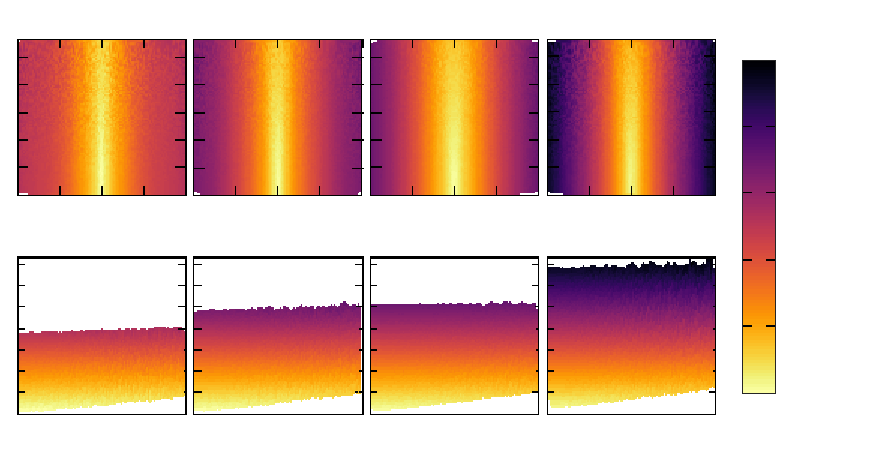
\includegraphics{./figures/parts/02/chapters/04/sections/04/caer_x2_sm0}}%
    \gplfronttext
  \end{picture}%
\endgroup

    \vspace{0.25cm}
    \caption{\small $\sigma_{\bm{M}} = 0.0$ m}
    \vspace{0.5cm}
  \end{subfigure}\\%
  \begin{subfigure}{\linewidth}\hspace{1cm}
    % GNUPLOT: LaTeX picture with Postscript
\begingroup
  \makeatletter
  \providecommand\color[2][]{%
    \GenericError{(gnuplot) \space\space\space\@spaces}{%
      Package color not loaded in conjunction with
      terminal option `colourtext'%
    }{See the gnuplot documentation for explanation.%
    }{Either use 'blacktext' in gnuplot or load the package
      color.sty in LaTeX.}%
    \renewcommand\color[2][]{}%
  }%
  \providecommand\includegraphics[2][]{%
    \GenericError{(gnuplot) \space\space\space\@spaces}{%
      Package graphicx or graphics not loaded%
    }{See the gnuplot documentation for explanation.%
    }{The gnuplot epslatex terminal needs graphicx.sty or graphics.sty.}%
    \renewcommand\includegraphics[2][]{}%
  }%
  \providecommand\rotatebox[2]{#2}%
  \@ifundefined{ifGPcolor}{%
    \newif\ifGPcolor
    \GPcolorfalse
  }{}%
  \@ifundefined{ifGPblacktext}{%
    \newif\ifGPblacktext
    \GPblacktexttrue
  }{}%
  % define a \g@addto@macro without @ in the name:
  \let\gplgaddtomacro\g@addto@macro
  % define empty templates for all commands taking text:
  \gdef\gplfronttext{}%
  \gdef\gplfronttext{}%
  \makeatother
  \ifGPblacktext
    % no textcolor at all
    \def\colorrgb#1{}%
    \def\colorgray#1{}%
  \else
    % gray or color?
    \ifGPcolor
      \def\colorrgb#1{\color[rgb]{#1}}%
      \def\colorgray#1{\color[gray]{#1}}%
      \expandafter\def\csname LTw\endcsname{\color{white}}%
      \expandafter\def\csname LTb\endcsname{\color{black}}%
      \expandafter\def\csname LTa\endcsname{\color{black}}%
      \expandafter\def\csname LT0\endcsname{\color[rgb]{1,0,0}}%
      \expandafter\def\csname LT1\endcsname{\color[rgb]{0,1,0}}%
      \expandafter\def\csname LT2\endcsname{\color[rgb]{0,0,1}}%
      \expandafter\def\csname LT3\endcsname{\color[rgb]{1,0,1}}%
      \expandafter\def\csname LT4\endcsname{\color[rgb]{0,1,1}}%
      \expandafter\def\csname LT5\endcsname{\color[rgb]{1,1,0}}%
      \expandafter\def\csname LT6\endcsname{\color[rgb]{0,0,0}}%
      \expandafter\def\csname LT7\endcsname{\color[rgb]{1,0.3,0}}%
      \expandafter\def\csname LT8\endcsname{\color[rgb]{0.5,0.5,0.5}}%
    \else
      % gray
      \def\colorrgb#1{\color{black}}%
      \def\colorgray#1{\color[gray]{#1}}%
      \expandafter\def\csname LTw\endcsname{\color{white}}%
      \expandafter\def\csname LTb\endcsname{\color{black}}%
      \expandafter\def\csname LTa\endcsname{\color{black}}%
      \expandafter\def\csname LT0\endcsname{\color{black}}%
      \expandafter\def\csname LT1\endcsname{\color{black}}%
      \expandafter\def\csname LT2\endcsname{\color{black}}%
      \expandafter\def\csname LT3\endcsname{\color{black}}%
      \expandafter\def\csname LT4\endcsname{\color{black}}%
      \expandafter\def\csname LT5\endcsname{\color{black}}%
      \expandafter\def\csname LT6\endcsname{\color{black}}%
      \expandafter\def\csname LT7\endcsname{\color{black}}%
      \expandafter\def\csname LT8\endcsname{\color{black}}%
    \fi
  \fi
    \setlength{\unitlength}{0.0500bp}%
    \ifx\gptboxheight\undefined%
      \newlength{\gptboxheight}%
      \newlength{\gptboxwidth}%
      \newsavebox{\gptboxtext}%
    \fi%
    \setlength{\fboxrule}{0.5pt}%
    \setlength{\fboxsep}{1pt}%
\begin{picture}(8000.00,4000.00)%
    \gplgaddtomacro\gplfronttext{%
    }%
    \gplgaddtomacro\gplfronttext{%
      \put(-404,2800){\rotatebox{90}{\strut{}$\|\Delta \bm{l}\|_2$}}%
      \put(3350,2025){\makebox(0,0){\strut{}Σφάλμα εκτίμησης προσανατολισμού $\Delta\theta \in [-\frac{\pi}{4}, +\frac{\pi}{4}]$ rad}}%
    }%
    \gplgaddtomacro\gplfronttext{%
      \put(808,3939){\makebox(0,0){\strut{}$\sigma_R = 0.0$ m}}%
      }
    \gplgaddtomacro\gplfronttext{%
      \put(2504,3939){\makebox(0,0){\strut{}$\sigma_R = 0.03$ m}}%
      }
    \gplgaddtomacro\gplfronttext{%
      \put(4199,3939){\makebox(0,0){\strut{}$\sigma_R = 0.05$ m}}%
      }
    \gplgaddtomacro\gplfronttext{%
      \put(5895,3939){\makebox(0,0){\strut{}$\sigma_R = 0.10$ m}}%
      }
    \gplgaddtomacro\gplfronttext{%
      \put(3350,-100){\makebox(0,0){\strut{}Μέτρο σφάλματος εκτίμησης θέσης $\|\Delta \bm{l}\|_2 \in [0.0, \sqrt{2}\cdot 0.2]$ m}}%
      \put(-304,950){\rotatebox{90}{\makebox(0,0){\strut{}CAER [m]}}}%
    }%
    \gplgaddtomacro\gplfronttext{%
      \colorrgb{0.15,0.15,0.15}%
      \put(7411,400){\makebox(0,0)[l]{\strut{}$0.0$}}%
      \colorrgb{0.15,0.15,0.15}%
      \put(7411,1040){\makebox(0,0)[l]{\strut{}$145.3$}}%
      \colorrgb{0.15,0.15,0.15}%
      \put(7411,1680){\makebox(0,0)[l]{\strut{}$290.6$}}%
      \colorrgb{0.15,0.15,0.15}%
      \put(7411,2319){\makebox(0,0)[l]{\strut{}$436.0$}}%
      \colorrgb{0.15,0.15,0.15}%
      \put(7411,2959){\makebox(0,0)[l]{\strut{}$581.3$}}%
      \colorrgb{0.15,0.15,0.15}%
      \put(7411,3599){\makebox(0,0)[l]{\strut{}$726.5$}}%
    }%
    \put(0,0){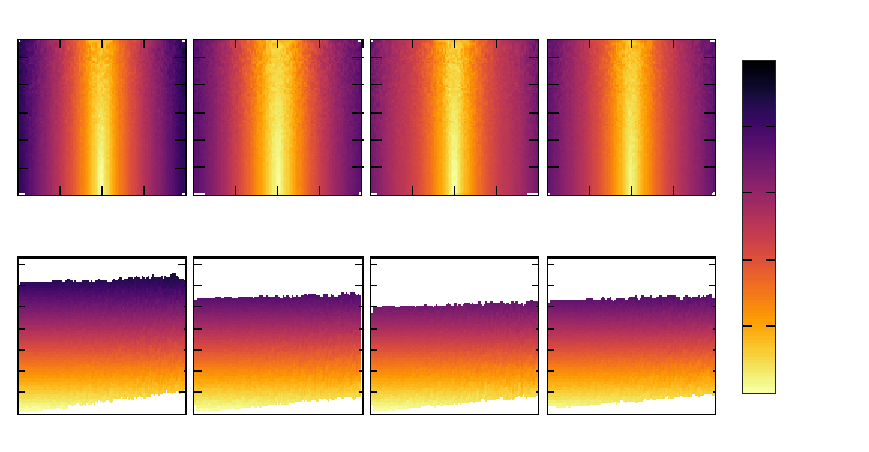
\includegraphics{./figures/parts/02/chapters/04/sections/04/caer_x2_sm5}}%
    \gplfronttext
  \end{picture}%
\endgroup

    \vspace{0.25cm}
    \caption{\small $\sigma_{\bm{M}} = 0.05$ m}
    \vspace{0.5cm}
  \end{subfigure}%
  \vspace{-0.25cm}
  \caption{\small Κατόψεις (πρώτη και τρίτη σειρά) και πλάγιες όψεις
           (δεύτερη και τέταρτη) της μετρικής CAER (εξίσωση
           \ref{eq:caer_normal}) από $10^5$ ζεύγη μίας σάρωσης σταθερής στάσης
           και εικονικών σαρώσεων που συνελήφθησαν από τυχαίες στάσεις, ανάλογα
           με την απόσταση $(\Delta x^2 + \Delta y^2)^{1/2}$, $\Delta x, \Delta
           y \in [-0.2, +0,2]$ m, και το σχετικού προσανατολισμό $\Delta \theta
           \in [-\pi/, +\pi/4]$ rad των στάσεων από όπου αυτές καταγράφηκαν,
           για αυξανόμενες τιμές της τυπικής απόκλισης των διαταραχών των
           πραγματικών μετρήσεων $\sigma_R$, και διαφθοράς του χαρτη
           $\sigma_{\bm{M}}$. Οι εκτιμήσεις στάσεις που είναι πιο κοντά στην
           πραγματική στάση από άποψη (α) προσανατολισμού και (β) θέσης
           παρουσιάζουν χαμηλότερες τιμές CAER από εκείνες που απέχουν
           περισσότερο από αυτήν}
  \label{fig:02_04_04:caer}
\end{figure}

Με την εισαγωγή της λειτουργίας δειγματοληψίας κατά Θησέα στη μέθοδο εκτίμησης
προσανατολισμού Πρώτων Αρχών, την αφαίρεση του υπολογισμού και σύγκρισης των
τιμών του Ποσοστού Διάκρισης, και την εισαγωγή της μετρικής CAER καταφέρνουμε
να χτυπήσουμε με ένα σμπάρο δύο τριγώνια για όλες τις μεθόδους εκτίμησης
προσανατολισμού, διότι με αυτόν τον τρόπο:

\begin{itemize}
  \item ιδρύουμε έναν ορθολογικό μηχανισμό σύγκρισης των
        εκτιμήσεων προσανατολισμού της μεθόδου εκτίμησης προσανατολισμού Πρώτων
        Αρχών (Παρατηρήσεις \ref{remark:02_04_02:02} και
        \ref{remark:02_04_02:03})
  \item παρακάμπτουμε τον ύφαλο που δημιουργεί η σύγκριση τους μέσω της μετρικής
        Ποσοστού Διάκρισης για τις Προκρούστειες μεθόδους σε συνθήκες ανισότητας
        θέσεων (Παρατήρηση \ref{remark:02_04_02:04} )
\end{itemize}

Καθώς κάθε μέθοδος εξάγει πλέον $2^\nu$ εκτιμήσεις προσανατολισμού, όλες με την
ίδια εκτίμηση θέσης, συλλαμβάνοντας από την κάθε μία εικονική σάρωση εντός του
$\bm{M}$ και εισάγοντας την στη μετρική CAER παράγει μία τιμή που αυξάνει για
αυξανόμενο σφάλμα προσανατολισμού (σχήμα \ref{fig:02_04_04:caer}, πρώτη και
τρίτη σειρά)---και αυτή η ιδιότητα διατηρείται στη γενική συνθήκη όπου οι
μετρήσεις του φυσικού αισθητήρα και η ταύτιση του χάρτη με το περιβάλλον που
αναπαριστά είναι διεφθαρμένες από θόρυβο.

Σε αυτό το σημείο έχουμε εκμεταλλευτεί μόνο την ιδιότητα της παρατήρησης
\ref{remark:02_04_02:01}. Για τον επιπρόσθετο διαχωρισμό ανάμεσα στις
εκτιμήσεις προσανατολισμού εκμεταλλευόμαστε την καμπυλότητα της CAER και την
ιδιότητα της παρατήρησης \ref{remark:loc_prop_or} με τον εξής τρόπο: δεδομένου
ότι εκτιμήσεις στάσης μεγαλύτερου σφάλματος  προσανατολισμού οδηγούν σε (α)
υψηλότερα σφάλματα θέσης όταν εισαχθούν στη μέθοδο εκτίμησης θέσης Πρώτων
Αρχών, και (β) υψηλότερες τιμές CAER, αν εισάγουμε τις $2^\nu$ εκτιμήσεις
στάσης που έχουν προέλθει από τις τρεις μεθόδους εκτίμησης προσανατολισμού στη
μέθοδο εκτίμησης θέσης για έναν περιορισμένο αριθμό επαναλήψεων, τότε οι
περισσότερο ανακριβείς ως προς τον προσανατολισμό στάσεις θα οδηγηθούν σε
περισσότερο ανακριβείς θέσεις, και, κατά συνέπεια, οι εικονικές σαρώσεις που
συλλαμβάνονται από αυτές θα οδηγήσουν σε μεγαλύτερες τιμές CAER σε σχέση με τις
λιγότερο ανακριβείς στάσεις κατά προσανατολισμό. Ταυτόχρονα, με αυτόν τον
τρόπο, γίνεται εφικτό να εισαχθεί μόνο μία εκτίμηση στάσης από τις $2^\nu$ στη
μέθοδο εκτίμησης θέσης (αυτή με τη χαμηλότερη τιμή CAER), με αποτέλεσμα
χαμηλότερο χρόνο εκτέλεσης της από κοινού μεθόδου ευθυγράμμισης.


\begin{figure}[!h]\centering
  

\tikzset{every picture/.style={line width=0.75pt}} %set default line width to 0.75pt

\begin{tikzpicture}[x=0.75pt,y=0.75pt,yscale=-1,xscale=1]
%uncomment if require: \path (0,542); %set diagram left start at 0, and has height of 542

%Straight Lines [id:da5372026622110897]
\draw    (126.5,63) -- (126.5,126.9) ;
%Straight Lines [id:da7972290663823844]
\draw    (260.5,64) -- (260.5,108) ;
\draw    (156.5,63) -- (156.5,266) ; % M top
\draw    (156.0,266) -- (195.5,266) ;
\draw [shift={(195.5,266)}, rotate = 180] [color={rgb, 255:red, 0; green, 0; blue, 0 }  ][line width=0.75]    (10.93,-3.29) .. controls (6.95,-1.4) and (3.31,-0.3) .. (0,0) .. controls (3.31,0.3) and (6.95,1.4) .. (10.93,3.29)   ;



\draw [shift={(260.5,110)}, rotate = 270] [color={rgb, 255:red, 0; green, 0; blue, 0 }  ][line width=0.75]    (10.93,-3.29) .. controls (6.95,-1.4) and (3.31,-0.3) .. (0,0) .. controls (3.31,0.3) and (6.95,1.4) .. (10.93,3.29)   ;
%Straight Lines [id:da2357744220142839]
\draw    (260.5,138.86) -- (260.5,167.86) ;
\draw [shift={(260.5,169.86)}, rotate = 270] [color={rgb, 255:red, 0; green, 0; blue, 0 }  ][line width=0.75]    (10.93,-3.29) .. controls (6.95,-1.4) and (3.31,-0.3) .. (0,0) .. controls (3.31,0.3) and (6.95,1.4) .. (10.93,3.29)   ;
%Straight Lines [id:da9232696254114303]
\draw    (372.5,193.29) -- (343,193.29) ;
\draw [shift={(343,193.29)}, rotate = 0] [color={rgb, 255:red, 0; green, 0; blue, 0 }  ][line width=0.75]    (10.93,-3.29) .. controls (6.95,-1.4) and (3.31,-0.3) .. (0,0) .. controls (3.31,0.3) and (6.95,1.4) .. (10.93,3.29)   ;
%Straight Lines [id:da7890748320756154]
\draw    (259.5,278.86) -- (259.5,311.86) ;
\draw [shift={(259.5,313.86)}, rotate = 270] [color={rgb, 255:red, 0; green, 0; blue, 0 }  ][line width=0.75]    (10.93,-3.29) .. controls (6.95,-1.4) and (3.31,-0.3) .. (0,0) .. controls (3.31,0.3) and (6.95,1.4) .. (10.93,3.29)   ;
%Straight Lines [id:da3579629949332166]
\draw    (260.5,342.86) -- (260.5,364.86) ;
\draw [shift={(260.5,366.86)}, rotate = 270] [color={rgb, 255:red, 0; green, 0; blue, 0 }  ][line width=0.75]    (10.93,-3.29) .. controls (6.95,-1.4) and (3.31,-0.3) .. (0,0) .. controls (3.31,0.3) and (6.95,1.4) .. (10.93,3.29)   ;
%Straight Lines [id:da8737381615370248]
\draw    (141.5,63) -- (141.5,329.29) ;
%Straight Lines [id:da6971384120103545]
%Straight Lines [id:da8422749343405824]
\draw    (178.5,126.4) -- (156.5,126.4) ;
\draw [shift={(156.5,126.4)}, rotate = 180] [color={rgb, 255:red, 0; green, 0; blue, 0 }  ][fill={rgb, 255:red, 0; green, 0; blue, 0 }  ][line width=0.75]      (0, 0) circle [x radius= 1.35, y radius= 1.35]   ;
\draw [shift={(180.5,126.4)}, rotate = 180] [color={rgb, 255:red, 0; green, 0; blue, 0 }  ][line width=0.75]    (10.93,-3.29) .. controls (6.95,-1.4) and (3.31,-0.3) .. (0,0) .. controls (3.31,0.3) and (6.95,1.4) .. (10.93,3.29)   ;
%Straight Lines [id:da4007753539436163]
\draw    (156.5,126.4) -- (141.5,126.4) ;
\draw [shift={(141.5,126.4)}, rotate = 180] [color={rgb, 255:red, 0; green, 0; blue, 0 }  ][fill={rgb, 255:red, 0; green, 0; blue, 0 }  ][line width=0.75]      (0, 0) circle [x radius= 1.35, y radius= 1.35]   ;
%Straight Lines [id:da579363628601445]
\draw    (141.5,126.4) -- (126.5,126.4) ;
%Straight Lines [id:da5833842782446357]
%\draw    (362.5,329.43) -- (338.5,329.43) ;
%\draw [shift={(338.5,329.43)}, rotate = 0] [color={rgb, 255:red, 0; green, 0; blue, 0 }  ][line width=0.75]    (10.93,-3.29) .. controls (6.95,-1.4) and (3.31,-0.3) .. (0,0) .. controls (3.31,0.3) and (6.95,1.4) .. (10.93,3.29)   ;
%Straight Lines [id:da7806442385955334]
\draw    (260.5,214.86) -- (260.5,246.86) ;
\draw [shift={(260.5,248.86)}, rotate = 270] [color={rgb, 255:red, 0; green, 0; blue, 0 }  ][line width=0.75]    (10.93,-3.29) .. controls (6.95,-1.4) and (3.31,-0.3) .. (0,0) .. controls (3.31,0.3) and (6.95,1.4) .. (10.93,3.29)   ;
%Straight Lines [id:da6458571735202372]
\draw    (194.5,194.4) -- (156.5,194.4) ;
\draw [shift={(156.5,194.4)}, rotate = 180] [color={rgb, 255:red, 0; green, 0; blue, 0 }  ][fill={rgb, 255:red, 0; green, 0; blue, 0 }  ][line width=0.75]      (0, 0) circle [x radius= 1.35, y radius= 1.35]   ;
\draw [shift={(196.5,194.4)}, rotate = 180] [color={rgb, 255:red, 0; green, 0; blue, 0 }  ][line width=0.75]    (10.93,-3.29) .. controls (6.95,-1.4) and (3.31,-0.3) .. (0,0) .. controls (3.31,0.3) and (6.95,1.4) .. (10.93,3.29)   ;
%Straight Lines [id:da3539392704501798]
\draw    (156.5,194.5) -- (141.5,194.5) ;
%Straight Lines [id:da41656320353747733]
\draw    (197.5,329.4) -- (141.0,329.4) ;
\draw [shift={(198.5,329.4)}, rotate = 180] [color={rgb, 255:red, 0; green, 0; blue, 0 }  ][line width=0.75]    (10.93,-3.29) .. controls (6.95,-1.4) and (3.31,-0.3) .. (0,0) .. controls (3.31,0.3) and (6.95,1.4) .. (10.93,3.29)   ;
%Shape: Rectangle [id:dp8185193791005427]
\draw  [dash pattern={on 0.84pt off 2.51pt}] (105,75) -- (420,75) -- (420,350) -- (105,350) -- cycle ;

\draw (379,45) node  {CAER-based};
\draw (379,63) node  {Orientation Estimation};

% Text Node
\draw    (184,114) -- (358,114) -- (358,139) -- (184,139) -- cycle  ;
\draw (189,120) node [anchor=north west][inner sep=0.75pt]   [align=left] {\ \ Orientation Estimation};
% Text Node
\draw (119,47) node [anchor=north west][inner sep=0.75pt]   [align=left] {$\nu$};
% Text Node
\draw (131,44) node [anchor=north west][inner sep=0.75pt]   [align=left] {$\mathcal{S}_{R}$};
% Text Node
\draw (258,40.57) node [anchor=north west][inner sep=0.75pt]   [align=left] {$\hat{\bm{p}}$};
% Text Node
\draw (150,44.57) node [anchor=north west][inner sep=0.75pt]   [align=left] {$\bm{M}$};
% Text Node
\draw  [color={rgb, 255:red, 0; green, 0; blue, 0 }  ,draw opacity=1 ]  (201,174) -- (341,174) -- (341,215) -- (201,215) -- cycle  ;
\draw (203,180) node [anchor=north west][inner sep=0.75pt]  [align=left] {\ \ \ \ \ \ \ Rehearsal \\ \ Position Estimation};
% Text Node
\draw    (196.5,253) -- (345.5,253) -- (345.5,279) -- (196.5,279) -- cycle  ;
\draw (235,259) node [anchor=north west][inner sep=0.75pt]   [align=left] {Scan Map};
% Text Node
\draw (376,187) node [anchor=north west][inner sep=0.75pt]   [align=left] {$I = 1$};
% Text Node
\draw    (199,317) -- (343,317) -- (343,342) -- (199,342) -- cycle  ;
% Text Node
% Text Node
\draw (271,145.5) node [anchor=north west][inner sep=0.75pt]   [align=left] {$\hat{\bm{P}}_{OC} = \text{OC}(\hat{\bm{p}})$};
% Text Node
\draw (271,223.5) node [anchor=north west][inner sep=0.75pt]   [align=left] {$\hat{\bm{P}}_{RPC} = \text{RPC}(\hat{\bm{P}}_{OC})$};
% Text Node
\draw (271,289.5) node [anchor=north west][inner sep=0.75pt]   [align=left] {$\bm{\mathcal{S}}_V$};
\draw (190,322) node [anchor=north west][inner sep=0.75pt]   [align=left] {\ \ \ $\bm{C} = \text{CAER}(\mathcal{S}_R, \bm{\mathcal{S}}_V)$};
\draw (73,372.67) node [anchor=north west][inner sep=0.75pt]   [align=left] {$\hat{\bm{p}}_{C} \in \hat{\bm{P}}_{OC} : \text{CAER}(\mathcal{S}_R, \texttt{scan\_map}(\bm{M}, \text{RPC}(\hat{\bm{p}}_C))) = \min\{\bm{C}\}$};


\end{tikzpicture}

  \caption{\small Το μπλοκ διάγραμμα του τελικού συστήματος εκτίμησης
           προσανατολισμού του συστήματος ευθυγράμμισης πραγματικών με εικονικές
           σαρώσεις, FSMSM}
  \label{fig:02_04_04:inner_rotation_system}
\end{figure}


\begin{algorithm}[!h]
  \caption{\texttt{caer-based\_orientation\_estimation}}
  \begin{spacing}{1.5}
  \begin{algorithmic}[1]
    \REQUIRE \texttt{rc}, $\bm{M}$, $\mathcal{S}_R$, $\hat{\bm{p}}(\hat{x}, \hat{y}, \hat{\theta})$, $\gamma$, $N_s$, $\nu$
    \ENSURE $\hat{\bm{p}}_C(\hat{x}, \hat{y}, \hat{\theta}_C)$
    \STATE \tikzmk{A}$\hat{\bm{P}}_{OE} \leftarrow \{\varnothing\}$
    \FOR{$k = 0 : 2^\nu-1$}
      \STATE $\hat{\bm{p}}_k \leftarrow (\hat{x}, \hat{y}, \hat{\theta} + k \cdot \gamma/2^\nu)$ \hfill (εξ. \ref{eq:theta_k_theseus})
      \STATE $\mathcal{S}_V^k \leftarrow \texttt{scan\_map}(\bm{M}, \hat{\bm{p}}_k, N_s)$ \hfill (αλγ. \ref{alg:scan_map})
      \STATE $\hat{\theta}^\prime \leftarrow \texttt{rcm}(\mathcal{S}_R, \mathcal{S}_V, \hat{\bm{p}}_k, \gamma)$ \hfill (αλγ. \ref{alg:02_04_04:rcm})
      \STATE $\hat{\theta}_k \leftarrow \hat{\theta}^\prime + k \cdot \gamma/2^\nu$
      \STATE $\texttt{append} \ \ (\hat{x}, \hat{y}, \hat{\theta}_k)$ to $\hat{\bm{P}}_{OE}$
      \STATE $k \leftarrow k + 1$
    \ENDFOR \tikzmk{B}\boxit{alg1}
    \STATE \tikzmk{A}$\hat{\bm{P}}_{RPE} \leftarrow \{\varnothing\}$
    \FOR{$k = 0 : 2^\nu-1$}
      \STATE $\hat{\bm{p}}_k^\prime \leftarrow \texttt{tc\_x1}(\bm{M}, \mathcal{S}_R, \hat{\bm{P}}_{OE}[k], 1, \infty, N_s)$ \hfill (αλγ. \ref{alg:icte})
      \STATE $\texttt{append} \ \ \hat{\bm{p}}_k^\prime$ to $\hat{\bm{P}}_{RPE}$
    \ENDFOR\tikzmk{B}\boxit{alg2}
    \STATE \tikzmk{A}$\bm{C} \leftarrow \{\varnothing\}$
    \FOR{$k = 0 : 2^\nu-1$}
      \STATE $\mathcal{S}_V^{k \prime} \leftarrow \texttt{scan\_map}(\bm{M}, \hat{\bm{P}}_{RPE}[k], N_s)$
      \STATE $\texttt{append} \ \ \texttt{CAER}(\mathcal{S}_R, \mathcal{S}_V^{k \prime})$ to $\bm{C}$ \hfill (εξ. \ref{eq:caer_normal})
    \ENDFOR\tikzmk{B}\boxit{alg3}
    \STATE $k_{\min} \leftarrow \arg\min \{\bm{C}\}$
    \STATE $\hat{\bm{p}}_C(\hat{x}, \hat{y}, \hat{\theta}_C) \leftarrow \hat{\bm{P}}_{OE}[k_{\min}]$
    \RETURN $\hat{\bm{p}}_C$
  \end{algorithmic}
  \end{spacing}
  \label{alg:02_04_04:rc}
\end{algorithm}


\begin{algorithm}[!h]
  \caption{\texttt{rcm}}
  \begin{spacing}{1.5}
  \begin{algorithmic}[1]
    \REQUIRE \texttt{rc}, $\mathcal{S}_R, \mathcal{S}_V, \hat{\bm{p}}(\hat{x}, \hat{y}, \hat{\theta}), \gamma$
    \ENSURE $\hat{\theta}^\prime$
    \IF{$\texttt{rc} = \texttt{rc\_fm}$}
      \STATE $(\hat{\theta}^\prime, \cdot) \leftarrow \texttt{rc\_fm}(\mathcal{S}_R, \mathcal{S}_V, \hat{\bm{p}}(\hat{x}, \hat{y}, \hat{\theta}), \gamma)$ \hfill (αλγ. \ref{alg:algorithm_fmrc})
    \ELSIF{$\texttt{rc} = \texttt{rc\_x1}$}
      \STATE $\hat{\theta}^\prime \leftarrow \texttt{rc\_x1}(\mathcal{S}_R, \mathcal{S}_V, \hat{\bm{p}}(\hat{x}, \hat{y}, \hat{\theta}))$ \hfill (αλγ. \ref{alg:algorithm_x1rc})
    \ELSIF{$\texttt{rc} = \texttt{rc\_uf}$}
      \STATE $(\hat{\theta}^\prime, \cdot) \leftarrow \texttt{rc\_uf}(\mathcal{S}_R, \mathcal{S}_V, \hat{\bm{p}}(\hat{x}, \hat{y}, \hat{\theta}), \gamma)$ \hfill (αλγ. \ref{alg:algorithm_ufrc})
    \ENDIF
    \RETURN $\hat{\theta}^\prime$
  \end{algorithmic}
  \end{spacing}
  \label{alg:02_04_04:rcm}
\end{algorithm}


Πιο συγκεκριμένα: έστω τα δεδομένα του Προβλήματος \ref{prob:02_04}.  Έστω
επίσης βαθμός δειγματοληψίας του χάρτη $\nu \in \mathbb{Z}_{\geq 0}$. Τότε το
τελικό σύστημα εκτίμησης προσανατολισμού CAER-based Orientation Estimation, το
οποίο απεικονίζεται σε μπλοκ διάγραμμα στο σχήμα
\ref{fig:02_04_04:inner_rotation_system} και σε ψευδοκώδικα στον Αλγόριθμο
\ref{alg:02_04_04:rc}, υπολογίζει πρώτα $2^\nu$ εκτιμήσεις στάσης, οι οποίες
αποτελούν διατεταγμένα στοιχεία του συνόλου $\hat{\bm{P}}_{OE} = \{(\hat{x},
\hat{y}, \hat{\theta}_k)\}$, $k = 0,\dots,2^\nu-1$.  Όλες οι στάσεις του
$\hat{\bm{P}}_{OE}$ έχουν ίσες εκτιμήσεις θέσης, αλλά διαφορετικές εκτιμήσεις
προσανατολισμού. Η τελική εκτίμηση προσανατολισμού για κάθε υποψήφια αρχική
εκτίμηση προσανατολισμού $\hat{\theta}_k = \hat{\theta} + k \cdot \gamma
/2^\nu$ μεσολαβείται χρησιμοποιώντας έναν από τους βασικούς αλγορίθμους των
ενοτήτων \ref{subsection:02_04_02:01}, \ref{subsection:02_04_02:02}, και
\ref{subsection:02_04_02:03}, και ο δείκτης $k$ είναι ο δείκτης που καθορίζει
τη διάταξή τους στο σύνολο $\hat{\bm{P}}_{OE}$.

Προκειμένου να δημιουργηθεί μία ευκρινώς διαχωρισμένη ιεραρχία τιμών μετρικών
αξιολόγησης του σφάλματος των εκτιμήσεων προσανατολισμού, κάθε εκτίμηση στάσης
του $\hat{\bm{P}}_{OE}$ μεταφέρεται στο σύστημα εκτίμησης θέσης, όπου η θέση
κάθε εκτίμησης στάσης μετατοπίζεται μία φορά ($I_T = 1$), σύμφωνα με τον
Αλγόριθμο \ref{alg:icte}. Αυτή η λειτουργία, η οποία συμβολίζεται με τον τελεστή
RPE$(\cdot)$ στο σχήμα \ref{fig:02_04_04:inner_rotation_system}, παράγει το
σύνολο $\hat{\bm{P}}_{RPE} = \{(\hat{x}_k, \hat{y}_k, \hat{\theta}_k)\}$,
$|\hat{\bm{P}}_{RPE}| = 2^\nu$.  Με την πρόβα εκτίμησης θέσης κάθε εκτίμησης
στάσης του $\hat{\bm{P}}_{OE}$ και την καταγραφή της τιμής CAER για κάθε μια
από τις μετατοπισμένες εκτιμήσεις στάσης του $\hat{\bm{P}_{RPE}}$, είναι
δυνατόν να καθοριστεί μια κατάταξη σφάλματος στάσης μεταξύ όλων των εκτιμήσεων
του συνόλου $\hat{\bm{P}}_{OE}$, και ταυτόχρονα να διατηρείται μόνο μία
εκτίμηση στάσης για την επόμενη επανάληψη της συνολικής μεθόδου
εκτίμησης.\footnote{Σε αντίθετη περίπτωση η διόρθωση της θέσης των $2^\nu$
εκτιμήσεων στάσης και η επανατροφοδότησή τους στο σύστημα θα προκαλούσε
εκθετικό κόστος σε χρόνο εκτέλεσης.} Η εκτίμηση στάσης $\hat{\bm{p}}_C \in
\hat{\bm{P}}_{OE}$ η οποία όταν μετατοπιστεί μία φορά καταγράφει την ελάχιστη
τιμή CAER μεταξύ όλων των παρομοίως μεταχειρισθέντων εκτιμήσεων στάσης του
$\hat{\bm{P}}_{OE}$ είναι αυτή που εξάγεται από το τελικό σύστημα εκτίμησης
προσανατολισμού.


%%%%%%%%%%%%%%%%%%%%%%%%%%%%%%%%%%%%%%%%%%%%%%%%%%%%%%%%%%%%%%%%%%%%%%%%%%%%%%%%
\subsection{Το σύστημα από κοινού ευθυγράμμισης}
\label{subsection:02_04_04:02}

Σε αυτή την ενότητα παρουσιάζουμε το τελικό γενικό σύστημα που στοχεύει στην
επίλυση του προβλήματος \ref{prob:02_04} και το είναι ικανό να ενσωματώσει τη
μέθοδο εκτίμησης προσανατολισμού της προηγούμενης ενότητας και τη μέθοδο
εκτίμησης θέσης (ενότητα \ref{section:02_04_03}). Το προτεινόμενο σύστημα
εκτιμά αρχικά τον προσανατολισμό του αισθητήρα (ισοδύναμα του ρομπότ στον οποίο
είναι προσαρτημένος---Παρατήρηση \ref{remark:smsm_benefit}), και στη συνέχεια
θέση του, ως προς το σύστημα συντεταγμένων του χάρτη $\bm{M}$. Ως συνέπεια της
παρατήρησης \ref{rem:iterative}, η διαδικασία επαναλαμβάνεται μέχρι την
ικανοποίηση συνθήκης τερματισμού. Η μέθοδος αυτή περιγράφεται στα ακόλουθα.

\begin{figure}[!h]\centering
  \tikzset{every picture/.style={line width=0.75pt}} %set default line width to 0.75pt

\begin{tikzpicture}[x=0.75pt,y=0.75pt,yscale=-0.5,xscale=0.5]
%uncomment if require: \path (0,542); %set diagram left start at 0, and has height of 542

\draw    (126.5,63) -- (126.5,187) ; % nu vertical
\draw    (141.5,63) -- (141.5,187) ; % S_R vertical line
\draw    (156.5,63) -- (156.5,187) ; % M vertical line
\draw    (307,64) -- (307,108) ; hat p vertical line

\draw [shift={(307,110)}, rotate = 270] [color={rgb, 255:red, 0; green, 0; blue, 0 }  ][line width=0.75]    (10.93,-3.29) .. controls (6.95,-1.4) and (3.31,-0.3) .. (0,0) .. controls (3.31,0.3) and (6.95,1.4) .. (10.93,3.29)   ; % hat p vertical arrow

\draw    (307,138.86) -- (307,167.86) ; % after caer based orientation box vertical line

\draw [shift={(307,169.86)}, rotate = 270] [color={rgb, 255:red, 0; green, 0; blue, 0 }  ][line width=0.75]    (10.93,-3.29) .. controls (6.95,-1.4) and (3.31,-0.3) .. (0,0) .. controls (3.31,0.3) and (6.95,1.4) .. (10.93,3.29)   ; % after caer based orientation box vertical arrow

\draw    (178.5,126.4) -- (156.5,126.4) ; % M horizontal line to CAER Based

\draw [shift={(156.5,126.4)}, rotate = 180] [color={rgb, 255:red, 0; green, 0; blue, 0 }  ][fill={rgb, 255:red, 0; green, 0; blue, 0 }  ][line width=0.75]      (0, 0) circle [x radius= 1.35, y radius= 1.35]   ; % M horizontal line to CAER based dot

\draw [shift={(180.5,126.4)}, rotate = 180] [color={rgb, 255:red, 0; green, 0; blue, 0 }  ][line width=0.75]    (10.93,-3.29) .. controls (6.95,-1.4) and (3.31,-0.3) .. (0,0) .. controls (3.31,0.3) and (6.95,1.4) .. (10.93,3.29)   ; % M horizontal arrow to caer based

\draw    (156.5,126.4) -- (141.5,126.4) ; % S_R horizontal line to caer based

\draw [shift={(141.5,126.4)}, rotate = 180] [color={rgb, 255:red, 0; green, 0; blue, 0 }  ][fill={rgb, 255:red, 0; green, 0; blue, 0 }  ][line width=0.75]      (0, 0) circle [x radius= 1.35, y radius= 1.35]   ; % S_R horizontal line to caer based dot

\draw    (141.5,126.4) -- (126.5,126.4) ; % nu to caer based line




\draw    (185.5,187) -- (126.0,187) ; % nu to S_R line to position estimation
\draw    (156.5,187) -- (141.5,187) ; % S_R to position estimation line
\draw    (235.0,187) -- (156.5,187) ; % M line to position estimation

\draw [shift={(156.5,187)}, rotate = 180] [color={rgb, 255:red, 0; green, 0; blue, 0 }  ][fill={rgb, 255:red, 0; green, 0; blue, 0 }  ][line width=0.75]      (0, 0) circle [x radius= 1.35, y radius= 1.35]   ; % M dot to position estimation
\draw [shift={(141.5,187)}, rotate = 180] [color={rgb, 255:red, 0; green, 0; blue, 0 }  ][fill={rgb, 255:red, 0; green, 0; blue, 0 }  ][line width=0.75]      (0, 0) circle [x radius= 1.35, y radius= 1.35]   ; % S_R dot to position estimation
\draw [shift={(235.0,187)}, rotate = 180] [color={rgb, 255:red, 0; green, 0; blue, 0 }  ][line width=0.75]    (10.93,-3.29) .. controls (6.95,-1.4) and (3.31,-0.3) .. (0,0) .. controls (3.31,0.3) and (6.95,1.4) .. (10.93,3.29)   ; % M arrow to position estimation



\draw (235,174) -- (379,174) -- (379,200) -- (235,200) -- cycle  ;
\draw (235,180) node [anchor=north west][inner sep=0.75pt]   [align=left] {\tiny \ \ Position Estimation};

\draw (425,179) node [anchor=north west][inner sep=0.75pt]   [align=left] {$I_T = f( \nu )$};
\draw (379,187) -- (415.5,187) ; % I = fn line to position estimation
\draw [shift={(379,187)}, rotate = 0] [color={rgb, 255:red, 0; green, 0; blue, 0 }  ][line width=0.75]    (10.93,-3.29) .. controls (6.95,-1.4) and (3.31,-0.3) .. (0,0) .. controls (3.31,0.3) and (6.95,1.4) .. (10.93,3.29)   ;% I = fn arrow to position estimation


\draw (320,147.5) node [anchor=north west][inner sep=0.75pt]   [align=left] {$\hat{\bm{p}}_{C}$};
\draw (307,240) node [anchor=north west][inner sep=0.75pt]   [align=left] {$\hat{\bm{p}}^{\prime }$};

\draw (307,200) -- (307,235) ; % p final vertical line
\draw [shift={(307,235)}, rotate = 270] [color={rgb, 255:red, 0; green, 0; blue, 0 }  ][line width=0.75]    (10.93,-3.29) .. controls (6.95,-1.4) and (3.31,-0.3) .. (0,0) .. controls (3.31,0.3) and (6.95,1.4) .. (10.93,3.29)   ; % p final vertical arrow



%Shape: Rectangle [id:dp8185193791005427]
\draw  [dash pattern={on 0.84pt off 2.51pt}] (105,75) -- (500,75) -- (500,215) -- (105,215) -- cycle ;
\draw (410,65) node  {\tiny One-step Pose Estimation};

% Text Node
\draw    (184,114) -- (430,114) -- (430,139) -- (184,139) -- cycle  ;
\draw (189,120) node [anchor=north west][inner sep=0.75pt]   [align=left] {\tiny CAER-based Orientation Estimation};
% Text Node
\draw (119,47) node [anchor=north west][inner sep=0.75pt]   [align=left] {\tiny \tiny $\nu$};
% Text Node
\draw (131,44) node [anchor=north west][inner sep=0.75pt]   [align=left] {\tiny $\mathcal{S}_{R}$};
% Text Node
\draw (307,40.57) node [anchor=north west][inner sep=0.75pt]   [align=left] {\tiny $\hat{\bm{p}}$};
% Text Node
\draw (150,44.57) node [anchor=north west][inner sep=0.75pt]   [align=left] {\tiny $\bm{M}$};


\end{tikzpicture}

  \caption{\small Η κεντρική μέθοδος εκτίμησης στάσης του FSMSM,
           One-step Pose Estimation}
  \label{fig:02_04_04:inner_system}
\end{figure}


\begin{figure}[!h]\centering
  

\tikzset{every picture/.style={line width=0.75pt}} %set default line width to 0.75pt

\begin{tikzpicture}[x=0.75pt,y=0.75pt,yscale=-0.5,xscale=0.5]
%uncomment if require: \path (0,1001); %set diagram left start at 0, and has height of 1001

%Flowchart: Decision [id:dp5485531374796404]
\draw[fill opacity=.25]  (240.5,167) -- (311.5,202) -- (240.5,237) -- (169.5,202) -- cycle ;
%Straight Lines [id:da5877536487984554]
\draw    (240.5,52.67) -- (240.5,108.67) ;
\draw [shift={(240.5,110.67)}, rotate = 270] [color={rgb, 255:red, 0; green, 0; blue, 0 }  ][line width=0.75]    (10.93,-3.29) .. controls (6.95,-1.4) and (3.31,-0.3) .. (0,0) .. controls (3.31,0.3) and (6.95,1.4) .. (10.93,3.29)   ;
%Straight Lines [id:da7274819726754627]
\draw    (240.5,237) -- (240.5,261.67) ;
\draw [shift={(240.5,263.67)}, rotate = 270] [color={rgb, 255:red, 0; green, 0; blue, 0 }  ][line width=0.75]    (10.93,-3.29) .. controls (6.95,-1.4) and (3.31,-0.3) .. (0,0) .. controls (3.31,0.3) and (6.95,1.4) .. (10.93,3.29)   ;
%Straight Lines [id:da7064477442798851]
\draw    (309.5,202) -- (382.5,202) -- (382.5,422) ;
\draw [shift={(382.5,423)}, rotate = 270.0] [color={rgb, 255:red, 0; green, 0; blue, 0 }  ][line width=0.75]    (10.93,-3.29) .. controls (6.95,-1.4) and (3.31,-0.3) .. (0,0) .. controls (3.31,0.3) and (6.95,1.4) .. (10.93,3.29)   ;
%Flowchart: Decision [id:dp1133428099178595]
\draw [ fill opacity=.25]  (240.5,266) -- (311.5,301) -- (240.5,336) -- (169.5,301) -- cycle ;
%Flowchart: Decision [id:dp5073654995853492]
\draw [ fill opacity=.25]  (239.5,422) -- (310.5,457) -- (239.5,492) -- (168.5,457) -- cycle ;
%Straight Lines [id:da1335991408375894]
\draw    (239.5,492) -- (239.5,533.67) ;
\draw [shift={(239.5,535.67)}, rotate = 270] [color={rgb, 255:red, 0; green, 0; blue, 0 }  ][line width=0.75]    (10.93,-3.29) .. controls (6.95,-1.4) and (3.31,-0.3) .. (0,0) .. controls (3.31,0.3) and (6.95,1.4) .. (10.93,3.29)   ;
%Straight Lines [id:da5471544644867792]
\draw    (234.5,82.67) -- (130.5,82.67) -- (130.5,517.33) ;
\draw [shift={(236.5,82.67)}, rotate = 180] [color={rgb, 255:red, 0; green, 0; blue, 0 }  ][line width=0.75]    (10.93,-3.29) .. controls (6.95,-1.4) and (3.31,-0.3) .. (0,0) .. controls (3.31,0.3) and (6.95,1.4) .. (10.93,3.29)   ;
%Straight Lines [id:da06493806045400974]
\draw    (310.5,457) -- (329,457.03) -- (332,457.03) ;
\draw [shift={(332,457)}, rotate = 539.01] [color={rgb, 255:red, 0; green, 0; blue, 0 }  ][line width=0.75]    (10.93,-3.29) .. controls (6.95,-1.4) and (3.31,-0.3) .. (0,0) .. controls (3.31,0.3) and (6.95,1.4) .. (10.93,3.29)   ;
%Straight Lines [id:da02699596164541651]
\draw    (240.5,137) -- (240.5,161.67) ;
\draw [shift={(240.5,163.67)}, rotate = 270] [color={rgb, 255:red, 0; green, 0; blue, 0 }  ][line width=0.75]    (10.93,-3.29) .. controls (6.95,-1.4) and (3.31,-0.3) .. (0,0) .. controls (3.31,0.3) and (6.95,1.4) .. (10.93,3.29)   ;
%Straight Lines [id:da5283272652442879]
\draw    (240.5,336) -- (240.5,360.67) ;
\draw [shift={(240.5,362.67)}, rotate = 270] [color={rgb, 255:red, 0; green, 0; blue, 0 }  ][line width=0.75]    (10.93,-3.29) .. controls (6.95,-1.4) and (3.31,-0.3) .. (0,0) .. controls (3.31,0.3) and (6.95,1.4) .. (10.93,3.29)   ;
%Straight Lines [id:da11468273552980146]
\draw    (239.5,392.33) -- (239.5,417) ;
\draw [shift={(239.5,419)}, rotate = 270] [color={rgb, 255:red, 0; green, 0; blue, 0 }  ][line width=0.75]    (10.93,-3.29) .. controls (6.95,-1.4) and (3.31,-0.3) .. (0,0) .. controls (3.31,0.3) and (6.95,1.4) .. (10.93,3.29)   ;
%Straight Lines [id:da44842589807001]
\draw    (169.5,301) -- (136,301) ;
\draw [shift={(134,300.67)}, rotate = 360] [color={rgb, 255:red, 0; green, 0; blue, 0 }  ][line width=0.75]    (10.93,-3.29) .. controls (6.95,-1.4) and (3.31,-0.3) .. (0,0) .. controls (3.31,0.3) and (6.95,1.4) .. (10.93,3.29)   ;
%Straight Lines [id:da5521661750319236]
\draw    (382,488.67) -- (382,517.33) -- (130.5,517.33) ;

% Text Node
\draw (161,113) -- (406,113) -- (406,138) -- (161,138) -- cycle  ;
\draw (164,116) node [anchor=north west][inner sep=0.75pt]   [align=center] {\tiny Σύστημα Άπαξ Εκτίμησης Στάσης};
% Text Node
\draw    (241.84, 37.33) circle [x radius= 24.75, y radius= 14.85]   ;
\draw (241.84,37.33) node   [align=left] {\tiny Start};
% Text Node
\draw (207,183) node [anchor=north west][inner sep=0.75pt]  [align=center] {\tiny Συνθήκες };
\draw (198,198) node [anchor=north west][inner sep=0.75pt]  [align=center] {\tiny επαναφοράς};
% Text Node
\draw (205,282) node [anchor=north west][inner sep=0.75pt]  [align=center] {\tiny Συνθήκες};
\draw (201,297) node [anchor=north west][inner sep=0.75pt]  [align=center] {\tiny σύγκλισης};
% Text Node
\draw    (334,427.67) -- (433,427.67) -- (433,487.67) -- (334,487.67) -- cycle  ;
\draw (341,431.67) node [anchor=north west][inner sep=0.75pt]  [align=center] {\tiny Παραγωγή};
\draw (341,445.67) node [anchor=north west][inner sep=0.75pt]  [align=center] {\tiny $\hat{\bm{p}}^\prime$ από $\hat{\bm{p}}$,};
\draw (341,468.67) node [anchor=north west][inner sep=0.75pt]  [align=center] {\tiny $\nu \leftarrow \nu_{\min}$};
% Text Node
\draw (324,182.33) node [anchor=north west][inner sep=0.75pt]   [align=left] {\tiny Y};
% Text Node
\draw (251,245.33) node [anchor=north west][inner sep=0.75pt]   [align=left] {\tiny N};
% Text Node
\draw    (218,366.67) -- (263,366.67) -- (263,392.67) -- (218,392.67) -- cycle  ;
\draw (221,371.67) node [anchor=north west][inner sep=0.75pt]   [align=center] {\tiny $\nu$++};
% Text Node
\draw (251,343.33) node [anchor=north west][inner sep=0.75pt]   [align=left] {\tiny Y};
% Text Node
\draw (252,74.57) node [anchor=north west][inner sep=0.75pt]   [align=left] {\tiny $\nu$, $\mathcal{S}_R$, $\bm{M}$, $\hat{\bm{p}}$};
% Text Node
\draw (205,436) node [anchor=north west][inner sep=0.75pt] [align=center] {\tiny Συνθήκες};
\draw (199,454) node [anchor=north west][inner sep=0.75pt] [align=center] {\tiny τερματισμού};
% Text Node
\draw    (239.93, 555.33) circle [x radius= 48.79, y radius= 14.85]   ;
\draw (239.93,555.33) node   [align=left] {\tiny Terminate};
% Text Node
\draw (147,276.33) node [anchor=north west][inner sep=0.75pt]   [align=left] {\tiny N};
% Text Node
\draw (251,399.33) node [anchor=north west][inner sep=0.75pt]   [align=left] {\tiny Y};
% Text Node
\draw (314,437.33) node [anchor=north west][inner sep=0.75pt]   [align=left] {\tiny N};
% Text Node
\draw (251,145.57) node [anchor=north west][inner sep=0.75pt]   [align=left] {\tiny $\hat{\bm{p}}^\prime$};
% Text Node
\draw (250,493.33) node [anchor=north west][inner sep=0.75pt]   [align=left] {\tiny Y};


\end{tikzpicture}


  \caption{\small Το διάγραμμα ροής του FSMSM. Η εκτέλεση αρχίζει με έναν αρχικό
           ελάχιστο βαθμό δειγματοληψίας του χάρτη $\nu_{\min}$, τη σάρωση
           $\mathcal{S}_R$ που καταγράφεται από τον φυσικό αισθητήρα, και το
           χάρτη $\bm{M}$ του περιβάλλοντος στο οποίο βρίσκεται το ρομπότ. Η
           αρχική εκτίμηση της στάσης παρέχεται από έναν παρατηρητή κατά τη
           διάρκεια εκτίμησης στάσης βάσει περιορισμένης αβεβαιότητος, ή με τη
           μορφή μιας υπόθεσης κατά τη διάρκεια εκτίμησης στάσης βάσει καθολικής
           αβεβαιότητος. Η εσωτερική μέθοδος One-step Pose Estimation (σχήμα
           \ref{fig:02_04_04:inner_system}) καλείται επαναληπτικά, ενημερώνοντας
           την εκτίμηση στάσης μέχρι να επιτευχθεί ένας μέγιστος βαθμός
           δειγματοληψίας και σύγκλιση της εκτίμησης}
  \label{fig:02_04_04:outer_system}
\end{figure}

Έστω οι προϋποθέσεις του προβλήματος \ref{prob:02_04}, δηλαδή η αρχική εκτίμηση
εισόδου $\hat{\bm{p}}(\hat{x}, \hat{y}, \hat{\theta})$, η πραγματική σάρωση
$\mathcal{S}_R$, και ο χάρτης $\bm{M}$. Τότε η μέθοδος ελάττωσης του συνολικού
σφάλματος εκτίμησης στάσης που προτείνουμε, την οποία ονομάζουμε Fourier
Scan--to--Map-Scan Matching (FSMSM) και η οποία παρουσιάζεται στο σχήμα
\ref{fig:02_04_04:outer_system}---η μέθοδος μειώνει το σφάλμα εκτίμησης με την
επαναληπτική εκτέλεση της διαδικασίας εκτίμησης στάσης ενός βήματος (One-step
Pose Estimation, OPE---σχήμα \ref{fig:02_04_04:inner_system}), μέχρι να
ικανοποιηθεί ένα σύνολο συνθηκών τερματισμού. Η FSMSM ξεκινά με ένα αρχικό
βαθμό δειγματοληψίας του χάρτη $\nu$ = $\nu_{\min}$. Η εκτίμηση της στάσης
εισόδου επεξεργάζεται από την OPE, και η έξοδός της $\hat{\bm{p}}^\prime$
εξετάζεται ως προς συνθήκες ανάκτησης και σύγκλισης. Εάν η προκύπτουσα εκτίμηση
στάσης βρεθεί εκτός του χάρτη $\bm{M}$ τότε δημιουργείται με τυχαίο τρόπο μια νέα
εκτίμηση από την αρχική εκτίμηση $\hat{\bm{p}}$, και η διαδικασία επανεκκινεί,
με αρχική εκτίμηση τη νέα. Εάν δεν παρατηρείται σημαντική διόρθωση της
εκτίμησης $\|\hat{\bm{p}}^\prime-\hat{\bm{p}}\|_2 < \varepsilon_{\delta p}$,
τότε ο βαθμός δειγματοληψίας του χάρτη $\nu$ αυξάνεται και η τελευταία εκτίμηση
της OPE της τροφοδοτείται ως νέα αρχική συνθήκη. Η αύξησή του βαθμού
δειγματοληψίας χρησιμεύει ως μέσο μείωσης του σφάλματος προσανατολισμού και
συνεπώς του σφάλματος εκτίμησης θέσης (Παρατηρήσεις \ref{remark:02_04_02:01}
και \ref{remark:loc_prop_or}). Διαφορετικά, η παραπάνω διαδικασία
επαναλαμβάνεται με νέα αρχική εκτίμηση την τελευταία της OPE έως ότου δεν
παρατηρηθεί σημαντική διόρθωση. Η διαδικασία επαναλαμβάνεται έως ότου
επιτευχθεί μέγιστος βαθμός δειγματοληψίας χάρτη $\nu$ = $\nu_{\max}$, οπότε η
FSMSM τερματίζει εάν πληρούται μια τελική συνθήκη. Αυτή η τελική συνθήκη
διευκολύνει την αποφυγή τοπικών μεγίστων. Στην περίπτωση που αυτή η συνθήκη δεν
ικανοποιείται, δημιουργείται και πάλι με τυχαίο τρόπο μία νέα στάση και η
διαδικασία επανεκκινεί.


Η κεντρική μέθοδος One-step Pose Estimation χρησιμοποιεί μέθοδο εκτίμησης
προσανατολισμού της ενότητας \ref{subsection:02_04_04:01} και τη μέθοδο
εκτίμησης θέσης της ενότητας \ref{section:02_04_03}.  Στην τελευταία ο αριθμός
των επαναλήψεων $I_T$ είναι αύξουσα συνάρτηση του βαθμού δειγματοληψίας του
χάρτη $\nu$ ($I_T = f(\nu)$ στο σχήμα
\ref{fig:02_04_04:inner_system}).\footnote{Η λογική της αλυσιδωτής σύνδεσης του
αριθμού των επαναλήψεων της με το βαθμό δειγματοληψίας του χάρτη $\nu$ είναι η
ακόλουθη. Δεδομένου ότι το σφάλμα προσανατολισμού είναι αντιστρόφως ανάλογο του
$\nu$, σε χαμηλούς βαθμούς δειγματοληψίας χάρτη, όταν το σφάλμα εκτίμησης θέσης
είναι στα υψηλότερά του επίπεδα, εάν ο αριθμός των επαναλήψεων ήταν υψηλός τότε
η εκτίμηση της θέσης θα ήταν ευάλωτη σε απόκλιση.  Επομένως ο αριθμός των
επαναλήψεων διατηρείται χαμηλός στα αρχικά στάδια έτσι ώστε να υπάρχει
ισορροπία μεταξύ της μείωσης του σφάλματος θέσης και της απόκλισης της
εκτίμησης θέσης. Σε υψηλότερες τιμές του $\nu$ το σφάλμα εκτίμησης
προσανατολισμού έχει μειωθεί, και στη συνέχεια η απόκλιση περιορίζεται ή/και
επιτυγχάνεται σε υψηλότερες τιμές επανάληψης $I_T$. Καθώς η εκτίμηση
προσανατολισμού γίνεται όλο και πιο ακριβής, το σύστημα εκτίμησης θέσης
αφήνεται να επαναλάβει τη διαδικασία του περισσότερες φορές ώστε να είναι
εφικτή η περαιτέρω μείωση του σφάλματος θέσης.} Το σύστημα εκτίμησης θέσης
παράγει την εκτίμηση στάσης $\hat{\bm{p}}^\prime$, η οποίο στη συνέχεια
τροφοδοτείται πίσω στο σύστημα εκτίμησης προσανατολισμού με τη μορφή της νέας
του εκτίμησης στάσης: $\hat{\bm{p}} \leftarrow \hat{\bm{p}}^\prime$. Στην
πράξη, το σύνολο στάσεων $\hat{\bm{P}}_{OE}$ συμπληρώνεται με μία στάση της
οποίας η θέση είναι ίση με $\hat{\bm{p}}$, και της οποίας ο προσανατολισμός
είναι ίσος με τον προσανατολισμό της $\hat{\bm{p}}_C$ που παράγει την ελάχιστη
τιμή CAER με την πάροδο του χρόνου. Αυτή η προσθήκη εισάγει μια μορφή μνήμης
στο σύστημα, η οποία το βοηθά στην αποφυγή αποκλίσεων και η οποία, ως εκ
τούτου, ωφελεί την ταχύτητα εκτέλεσης.



\begin{figure}[!h]
  \begin{subfigure}{\linewidth}\hspace{-0.25cm}
    % GNUPLOT: LaTeX picture with Postscript
\begingroup
  \makeatletter
  \providecommand\color[2][]{%
    \GenericError{(gnuplot) \space\space\space\@spaces}{%
      Package color not loaded in conjunction with
      terminal option `colourtext'%
    }{See the gnuplot documentation for explanation.%
    }{Either use 'blacktext' in gnuplot or load the package
      color.sty in LaTeX.}%
    \renewcommand\color[2][]{}%
  }%
  \providecommand\includegraphics[2][]{%
    \GenericError{(gnuplot) \space\space\space\@spaces}{%
      Package graphicx or graphics not loaded%
    }{See the gnuplot documentation for explanation.%
    }{The gnuplot epslatex terminal needs graphicx.sty or graphics.sty.}%
    \renewcommand\includegraphics[2][]{}%
  }%
  \providecommand\rotatebox[2]{#2}%
  \@ifundefined{ifGPcolor}{%
    \newif\ifGPcolor
    \GPcolorfalse
  }{}%
  \@ifundefined{ifGPblacktext}{%
    \newif\ifGPblacktext
    \GPblacktexttrue
  }{}%
  % define a \g@addto@macro without @ in the name:
  \let\gplgaddtomacro\g@addto@macro
  % define empty templates for all commands taking text:
  \gdef\gplfronttext{}%
  \gdef\gplfronttext{}%
  \makeatother
  \ifGPblacktext
    % no textcolor at all
    \def\colorrgb#1{}%
    \def\colorgray#1{}%
  \else
    % gray or color?
    \ifGPcolor
      \def\colorrgb#1{\color[rgb]{#1}}%
      \def\colorgray#1{\color[gray]{#1}}%
      \expandafter\def\csname LTw\endcsname{\color{white}}%
      \expandafter\def\csname LTb\endcsname{\color{black}}%
      \expandafter\def\csname LTa\endcsname{\color{black}}%
      \expandafter\def\csname LT0\endcsname{\color[rgb]{1,0,0}}%
      \expandafter\def\csname LT1\endcsname{\color[rgb]{0,1,0}}%
      \expandafter\def\csname LT2\endcsname{\color[rgb]{0,0,1}}%
      \expandafter\def\csname LT3\endcsname{\color[rgb]{1,0,1}}%
      \expandafter\def\csname LT4\endcsname{\color[rgb]{0,1,1}}%
      \expandafter\def\csname LT5\endcsname{\color[rgb]{1,1,0}}%
      \expandafter\def\csname LT6\endcsname{\color[rgb]{0,0,0}}%
      \expandafter\def\csname LT7\endcsname{\color[rgb]{1,0.3,0}}%
      \expandafter\def\csname LT8\endcsname{\color[rgb]{0.5,0.5,0.5}}%
    \else
      % gray
      \def\colorrgb#1{\color{black}}%
      \def\colorgray#1{\color[gray]{#1}}%
      \expandafter\def\csname LTw\endcsname{\color{white}}%
      \expandafter\def\csname LTb\endcsname{\color{black}}%
      \expandafter\def\csname LTa\endcsname{\color{black}}%
      \expandafter\def\csname LT0\endcsname{\color{black}}%
      \expandafter\def\csname LT1\endcsname{\color{black}}%
      \expandafter\def\csname LT2\endcsname{\color{black}}%
      \expandafter\def\csname LT3\endcsname{\color{black}}%
      \expandafter\def\csname LT4\endcsname{\color{black}}%
      \expandafter\def\csname LT5\endcsname{\color{black}}%
      \expandafter\def\csname LT6\endcsname{\color{black}}%
      \expandafter\def\csname LT7\endcsname{\color{black}}%
      \expandafter\def\csname LT8\endcsname{\color{black}}%
    \fi
  \fi
    \setlength{\unitlength}{0.0500bp}%
    \ifx\gptboxheight\undefined%
      \newlength{\gptboxheight}%
      \newlength{\gptboxwidth}%
      \newsavebox{\gptboxtext}%
    \fi%
    \setlength{\fboxrule}{0.5pt}%
    \setlength{\fboxsep}{1pt}%
\begin{picture}(8000.00,2600.00)%
    \gplgaddtomacro\gplfronttext{%
      \colorrgb{0.15,0.15,0.15}%
      \put(1425,260){\makebox(0,0)[r]{\strut{}\small $1.0$}}%
      \colorrgb{0.15,0.15,0.15}%
      \put(1425,854){\makebox(0,0)[r]{\strut{}\small $2.0$}}%
      \colorrgb{0.15,0.15,0.15}%
      \put(1425,1448){\makebox(0,0)[r]{\strut{}\small $3.0$}}%
      \colorrgb{0.15,0.15,0.15}%
      \put(1425,2042){\makebox(0,0)[r]{\strut{}\small $4.0$}}%
      \colorrgb{0.15,0.15,0.15}%
      \colorrgb{0.15,0.15,0.15}%
      \put(1854,40){\makebox(0,0){\strut{}\small $-1.0$}}%
      \colorrgb{0.15,0.15,0.15}%
      \put(2448,40){\makebox(0,0){\strut{}\small $0.0$}}%
      \colorrgb{0.15,0.15,0.15}%
      \put(3042,40){\makebox(0,0){\strut{}\small $1.0$}}%
    }%
    \gplgaddtomacro\gplfronttext{%
      \colorrgb{0.00,0.00,0.00}%
      \put(2299,2559){\makebox(0,0){\strut{}Ευκλείδειος χώρος}}%
    }%
    \gplgaddtomacro\gplfronttext{%
      \colorrgb{0.15,0.15,0.15}%
      \put(4492,618){\makebox(0,0)[r]{\strut{}\small $-2.0$}}%
      \colorrgb{0.15,0.15,0.15}%
      \put(4492,1096){\makebox(0,0)[r]{\strut{}\small $-1.0$}}%
      \colorrgb{0.15,0.15,0.15}%
      \put(4492,1574){\makebox(0,0)[r]{\strut{}\small $0$}}%
      \colorrgb{0.15,0.15,0.15}%
      \put(4492,2052){\makebox(0,0)[r]{\strut{}\small $1.0$}}%
      \colorrgb{0.15,0.15,0.15}%
      \put(4863,40){\makebox(0,0){\strut{}\small $-2.0$}}%
      \colorrgb{0.15,0.15,0.15}%
      \put(5341,40){\makebox(0,0){\strut{}\small $-1.0$}}%
      \colorrgb{0.15,0.15,0.15}%
      \put(5819,40){\makebox(0,0){\strut{}\small $0$}}%
      \colorrgb{0.15,0.15,0.15}%
      \put(6297,40){\makebox(0,0){\strut{}\small $1.0$}}%
      \colorrgb{0.15,0.15,0.15}%
      \put(6775,40){\makebox(0,0){\strut{}\small $2.0$}}%
    }%
    \gplgaddtomacro\gplfronttext{%
      \colorrgb{0.00,0.00,0.00}%
      \put(5699,2559){\makebox(0,0){\strut{}Μετρήσεων χώρος}}%
    }%
    \put(0,0){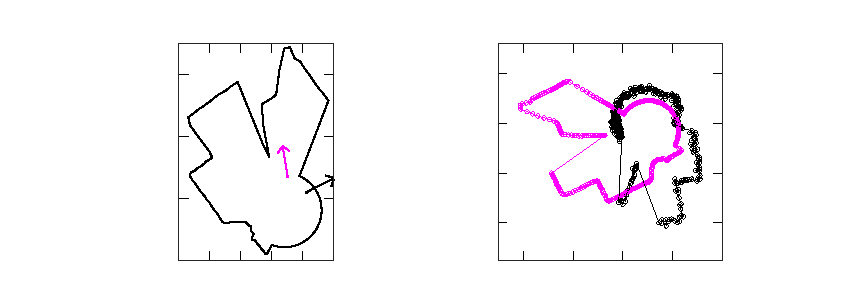
\includegraphics{./figures/parts/02/chapters/04/sections/04/sr5_sm0_0}}%
    \gplfronttext
  \end{picture}%
\endgroup

  \end{subfigure}\\%
  \begin{center}\vspace{-0.5cm}
    \hfill \texttt{FSMSM}\vspace{-0.5cm}
  \end{center}
  \begin{framed}
    \begin{subfigure}{\linewidth}\hspace{-0.25cm}
    % GNUPLOT: LaTeX picture with Postscript
\begingroup
  \makeatletter
  \providecommand\color[2][]{%
    \GenericError{(gnuplot) \space\space\space\@spaces}{%
      Package color not loaded in conjunction with
      terminal option `colourtext'%
    }{See the gnuplot documentation for explanation.%
    }{Either use 'blacktext' in gnuplot or load the package
      color.sty in LaTeX.}%
    \renewcommand\color[2][]{}%
  }%
  \providecommand\includegraphics[2][]{%
    \GenericError{(gnuplot) \space\space\space\@spaces}{%
      Package graphicx or graphics not loaded%
    }{See the gnuplot documentation for explanation.%
    }{The gnuplot epslatex terminal needs graphicx.sty or graphics.sty.}%
    \renewcommand\includegraphics[2][]{}%
  }%
  \providecommand\rotatebox[2]{#2}%
  \@ifundefined{ifGPcolor}{%
    \newif\ifGPcolor
    \GPcolorfalse
  }{}%
  \@ifundefined{ifGPblacktext}{%
    \newif\ifGPblacktext
    \GPblacktexttrue
  }{}%
  % define a \g@addto@macro without @ in the name:
  \let\gplgaddtomacro\g@addto@macro
  % define empty templates for all commands taking text:
  \gdef\gplfronttext{}%
  \gdef\gplfronttext{}%
  \makeatother
  \ifGPblacktext
    % no textcolor at all
    \def\colorrgb#1{}%
    \def\colorgray#1{}%
  \else
    % gray or color?
    \ifGPcolor
      \def\colorrgb#1{\color[rgb]{#1}}%
      \def\colorgray#1{\color[gray]{#1}}%
      \expandafter\def\csname LTw\endcsname{\color{white}}%
      \expandafter\def\csname LTb\endcsname{\color{black}}%
      \expandafter\def\csname LTa\endcsname{\color{black}}%
      \expandafter\def\csname LT0\endcsname{\color[rgb]{1,0,0}}%
      \expandafter\def\csname LT1\endcsname{\color[rgb]{0,1,0}}%
      \expandafter\def\csname LT2\endcsname{\color[rgb]{0,0,1}}%
      \expandafter\def\csname LT3\endcsname{\color[rgb]{1,0,1}}%
      \expandafter\def\csname LT4\endcsname{\color[rgb]{0,1,1}}%
      \expandafter\def\csname LT5\endcsname{\color[rgb]{1,1,0}}%
      \expandafter\def\csname LT6\endcsname{\color[rgb]{0,0,0}}%
      \expandafter\def\csname LT7\endcsname{\color[rgb]{1,0.3,0}}%
      \expandafter\def\csname LT8\endcsname{\color[rgb]{0.5,0.5,0.5}}%
    \else
      % gray
      \def\colorrgb#1{\color{black}}%
      \def\colorgray#1{\color[gray]{#1}}%
      \expandafter\def\csname LTw\endcsname{\color{white}}%
      \expandafter\def\csname LTb\endcsname{\color{black}}%
      \expandafter\def\csname LTa\endcsname{\color{black}}%
      \expandafter\def\csname LT0\endcsname{\color{black}}%
      \expandafter\def\csname LT1\endcsname{\color{black}}%
      \expandafter\def\csname LT2\endcsname{\color{black}}%
      \expandafter\def\csname LT3\endcsname{\color{black}}%
      \expandafter\def\csname LT4\endcsname{\color{black}}%
      \expandafter\def\csname LT5\endcsname{\color{black}}%
      \expandafter\def\csname LT6\endcsname{\color{black}}%
      \expandafter\def\csname LT7\endcsname{\color{black}}%
      \expandafter\def\csname LT8\endcsname{\color{black}}%
    \fi
  \fi
    \setlength{\unitlength}{0.0500bp}%
    \ifx\gptboxheight\undefined%
      \newlength{\gptboxheight}%
      \newlength{\gptboxwidth}%
      \newsavebox{\gptboxtext}%
    \fi%
    \setlength{\fboxrule}{0.5pt}%
    \setlength{\fboxsep}{1pt}%
\begin{picture}(8000.00,7000.00)%
    \gplgaddtomacro\gplfronttext{%
    }%
    \gplgaddtomacro\gplfronttext{%
    }%
    \gplgaddtomacro\gplfronttext{%
    }%
    \gplgaddtomacro\gplfronttext{%
      \colorrgb{0.00,0.00,0.00}%
      \put(1509,7049){\makebox(0,0){\strut{}\small Περιστροφή 1}}%
    }%
    \gplgaddtomacro\gplfronttext{%
      \colorrgb{0.00,0.45,0.74}%
      \put(2381,5782){\makebox(0,0)[r]{\strut{}\scriptsize $0.4$}}%
      \colorrgb{0.00,0.45,0.74}%
      \put(2381,6011){\makebox(0,0)[r]{\strut{}\scriptsize $0.6$}}%
      \colorrgb{0.00,0.45,0.74}%
      \put(2381,6241){\makebox(0,0)[r]{\strut{}\scriptsize $0.8$}}%
      \colorrgb{0.00,0.45,0.74}%
      \put(2381,6470){\makebox(0,0)[r]{\strut{}\scriptsize $1.0$}}%
      \colorrgb{0.00,0.45,0.74}%
      \put(2381,6700){\makebox(0,0)[r]{\strut{}\scriptsize $1.2$}}%
      \colorrgb{0.00,0.45,0.74}%
      \put(2381,6929){\makebox(0,0)[r]{\strut{}\scriptsize $1.4$}}%
      \colorrgb{0.15,0.15,0.15}%
      \put(2413,5662){\makebox(0,0){\strut{}\scriptsize $0$}}%
      \colorrgb{0.15,0.15,0.15}%
      \put(3739,5662){\makebox(0,0){\strut{}\scriptsize $0.5$}}%
    }%
    \gplgaddtomacro\gplfronttext{%
    }%
    \gplgaddtomacro\gplfronttext{%
      \colorrgb{0.85,0.33,0.10}%
      \put(3771,6069){\makebox(0,0)[l]{\strut{}\scriptsize $150$}}%
      \colorrgb{0.85,0.33,0.10}%
      \put(3771,6547){\makebox(0,0)[l]{\strut{}\scriptsize $200$}}%
    }%
    \gplgaddtomacro\gplfronttext{%
    }%
    \gplgaddtomacro\gplfronttext{%
    }%
    \gplgaddtomacro\gplfronttext{%
    }%
    \gplgaddtomacro\gplfronttext{%
    }%
    \gplgaddtomacro\gplfronttext{%
      \colorrgb{0.00,0.00,0.00}%
      \put(5489,7049){\makebox(0,0){\strut{}\small Μετατόπιση 1}}%
    }%
    \gplgaddtomacro\gplfronttext{%
      \colorrgb{0.00,0.45,0.74}%
      \put(6501,5782){\makebox(0,0)[r]{\strut{}\scriptsize $0.2$}}%
      \colorrgb{0.00,0.45,0.74}%
      \put(6501,5973){\makebox(0,0)[r]{\strut{}\scriptsize $0.4$}}%
      \colorrgb{0.00,0.45,0.74}%
      \put(6501,6164){\makebox(0,0)[r]{\strut{}\scriptsize $0.6$}}%
      \colorrgb{0.00,0.45,0.74}%
      \put(6501,6356){\makebox(0,0)[r]{\strut{}\scriptsize $0.8$}}%
      \colorrgb{0.00,0.45,0.74}%
      \put(6501,6547){\makebox(0,0)[r]{\strut{}\scriptsize $1.0$}}%
      \colorrgb{0.00,0.45,0.74}%
      \put(6501,6738){\makebox(0,0)[r]{\strut{}\scriptsize $1.2$}}%
      \colorrgb{0.00,0.45,0.74}%
      \put(6501,6929){\makebox(0,0)[r]{\strut{}\scriptsize $1.4$}}%
      \colorrgb{0.15,0.15,0.15}%
      \put(6633,5662){\makebox(0,0){\strut{}\scriptsize $0$}}%
      \colorrgb{0.15,0.15,0.15}%
      \put(7959,5662){\makebox(0,0){\strut{}\scriptsize $1$}}%
    }%
    \gplgaddtomacro\gplfronttext{%
    }%
    \gplgaddtomacro\gplfronttext{%
      \colorrgb{0.85,0.33,0.10}%
      \put(7991,5782){\makebox(0,0)[l]{\strut{}\scriptsize $50$}}%
      \colorrgb{0.85,0.33,0.10}%
      \put(7991,6069){\makebox(0,0)[l]{\strut{}\scriptsize $100$}}%
      \colorrgb{0.85,0.33,0.10}%
      \put(7991,6356){\makebox(0,0)[l]{\strut{}\scriptsize $150$}}%
      \colorrgb{0.85,0.33,0.10}%
      \put(7991,6642){\makebox(0,0)[l]{\strut{}\scriptsize $200$}}%
      \colorrgb{0.85,0.33,0.10}%
      \put(7991,6929){\makebox(0,0)[l]{\strut{}\scriptsize $250$}}%
    }%
    \gplgaddtomacro\gplfronttext{%
    }%
    \gplgaddtomacro\gplfronttext{%
    }%
    \gplgaddtomacro\gplfronttext{%
    }%
    \gplgaddtomacro\gplfronttext{%
    }%
    \gplgaddtomacro\gplfronttext{%
      \colorrgb{0.00,0.00,0.00}%
      \put(1429,5621){\makebox(0,0){\strut{}\small Περιστροφή 3}}%
    }%
    \gplgaddtomacro\gplfronttext{%
      \colorrgb{0.00,0.45,0.74}%
      \put(2381,4354){\makebox(0,0)[r]{\strut{}\scriptsize $0.0$}}%
      \colorrgb{0.00,0.45,0.74}%
      \put(2381,4518){\makebox(0,0)[r]{\strut{}\scriptsize $0.2$}}%
      \colorrgb{0.00,0.45,0.74}%
      \put(2381,4682){\makebox(0,0)[r]{\strut{}\scriptsize $0.4$}}%
      \colorrgb{0.00,0.45,0.74}%
      \put(2381,4846){\makebox(0,0)[r]{\strut{}\scriptsize $0.6$}}%
      \colorrgb{0.00,0.45,0.74}%
      \put(2381,5009){\makebox(0,0)[r]{\strut{}\scriptsize $0.8$}}%
      \colorrgb{0.00,0.45,0.74}%
      \put(2381,5173){\makebox(0,0)[r]{\strut{}\scriptsize $1.0$}}%
      \colorrgb{0.00,0.45,0.74}%
      \put(2381,5337){\makebox(0,0)[r]{\strut{}\scriptsize $1.2$}}%
      \colorrgb{0.00,0.45,0.74}%
      \put(2381,5501){\makebox(0,0)[r]{\strut{}\scriptsize $1.4$}}%
      \colorrgb{0.15,0.15,0.15}%
      \put(2413,4234){\makebox(0,0){\strut{}\scriptsize $0$}}%
      \colorrgb{0.15,0.15,0.15}%
      \put(2943,4234){\makebox(0,0){\strut{}\scriptsize $1$}}%
      \colorrgb{0.15,0.15,0.15}%
      \put(3474,4234){\makebox(0,0){\strut{}\scriptsize $2$}}%
    }%
    \gplgaddtomacro\gplfronttext{%
    }%
    \gplgaddtomacro\gplfronttext{%
      \colorrgb{0.85,0.33,0.10}%
      \put(3771,4354){\makebox(0,0)[l]{\strut{}\scriptsize $0$}}%
      \colorrgb{0.85,0.33,0.10}%
      \put(3771,4583){\makebox(0,0)[l]{\strut{}\scriptsize $50$}}%
      \colorrgb{0.85,0.33,0.10}%
      \put(3771,4813){\makebox(0,0)[l]{\strut{}\scriptsize $100$}}%
      \colorrgb{0.85,0.33,0.10}%
      \put(3771,5042){\makebox(0,0)[l]{\strut{}\scriptsize $150$}}%
      \colorrgb{0.85,0.33,0.10}%
      \put(3771,5272){\makebox(0,0)[l]{\strut{}\scriptsize $200$}}%
      \colorrgb{0.85,0.33,0.10}%
      \put(3771,5501){\makebox(0,0)[l]{\strut{}\scriptsize $250$}}%
    }%
    \gplgaddtomacro\gplfronttext{%
    }%
    \gplgaddtomacro\gplfronttext{%
    }%
    \gplgaddtomacro\gplfronttext{%
    }%
    \gplgaddtomacro\gplfronttext{%
    }%
    \gplgaddtomacro\gplfronttext{%
      \colorrgb{0.00,0.00,0.00}%
      \put(5529,5621){\makebox(0,0){\strut{}\small Μετατόπιση 3}}%
    }%
    \gplgaddtomacro\gplfronttext{%
      \colorrgb{0.00,0.45,0.74}%
      \put(6601,4354){\makebox(0,0)[r]{\strut{}\scriptsize $0.0$}}%
      \colorrgb{0.00,0.45,0.74}%
      \put(6601,4518){\makebox(0,0)[r]{\strut{}\scriptsize $0.2$}}%
      \colorrgb{0.00,0.45,0.74}%
      \put(6601,4682){\makebox(0,0)[r]{\strut{}\scriptsize $0.4$}}%
      \colorrgb{0.00,0.45,0.74}%
      \put(6601,4846){\makebox(0,0)[r]{\strut{}\scriptsize $0.6$}}%
      \colorrgb{0.00,0.45,0.74}%
      \put(6601,5009){\makebox(0,0)[r]{\strut{}\scriptsize $0.8$}}%
      \colorrgb{0.00,0.45,0.74}%
      \put(6601,5173){\makebox(0,0)[r]{\strut{}\scriptsize $1.0$}}%
      \colorrgb{0.00,0.45,0.74}%
      \put(6601,5337){\makebox(0,0)[r]{\strut{}\scriptsize $1.2$}}%
      \colorrgb{0.00,0.45,0.74}%
      \put(6601,5501){\makebox(0,0)[r]{\strut{}\scriptsize $1.4$}}%
      \colorrgb{0.15,0.15,0.15}%
      \put(6633,4234){\makebox(0,0){\strut{}\scriptsize $0$}}%
      \colorrgb{0.15,0.15,0.15}%
      \put(7075,4234){\makebox(0,0){\strut{}\scriptsize $1$}}%
      \colorrgb{0.15,0.15,0.15}%
      \put(7517,4234){\makebox(0,0){\strut{}\scriptsize $2$}}%
      \colorrgb{0.15,0.15,0.15}%
      \put(7959,4234){\makebox(0,0){\strut{}\scriptsize $3$}}%
    }%
    \gplgaddtomacro\gplfronttext{%
    }%
    \gplgaddtomacro\gplfronttext{%
      \colorrgb{0.85,0.33,0.10}%
      \put(7991,4354){\makebox(0,0)[l]{\strut{}\scriptsize $0$}}%
      \colorrgb{0.85,0.33,0.10}%
      \put(7991,4583){\makebox(0,0)[l]{\strut{}\scriptsize $50$}}%
      \colorrgb{0.85,0.33,0.10}%
      \put(7991,4813){\makebox(0,0)[l]{\strut{}\scriptsize $100$}}%
      \colorrgb{0.85,0.33,0.10}%
      \put(7991,5042){\makebox(0,0)[l]{\strut{}\scriptsize $150$}}%
      \colorrgb{0.85,0.33,0.10}%
      \put(7991,5272){\makebox(0,0)[l]{\strut{}\scriptsize $200$}}%
      \colorrgb{0.85,0.33,0.10}%
      \put(7991,5501){\makebox(0,0)[l]{\strut{}\scriptsize $250$}}%
    }%
    \gplgaddtomacro\gplfronttext{%
    }%
    \gplgaddtomacro\gplfronttext{%
    }%
    \gplgaddtomacro\gplfronttext{%
    }%
    \gplgaddtomacro\gplfronttext{%
    }%
    \gplgaddtomacro\gplfronttext{%
      \colorrgb{0.00,0.00,0.00}%
      \put(1429,4193){\makebox(0,0){\strut{}\small Περιστροφή 5}}%
    }%
    \gplgaddtomacro\gplfronttext{%
      \colorrgb{0.00,0.45,0.74}%
      \put(2381,2926){\makebox(0,0)[r]{\strut{}\scriptsize $0.0$}}%
      \colorrgb{0.00,0.45,0.74}%
      \put(2381,3090){\makebox(0,0)[r]{\strut{}\scriptsize $0.2$}}%
      \colorrgb{0.00,0.45,0.74}%
      \put(2381,3254){\makebox(0,0)[r]{\strut{}\scriptsize $0.4$}}%
      \colorrgb{0.00,0.45,0.74}%
      \put(2381,3418){\makebox(0,0)[r]{\strut{}\scriptsize $0.6$}}%
      \colorrgb{0.00,0.45,0.74}%
      \put(2381,3581){\makebox(0,0)[r]{\strut{}\scriptsize $0.8$}}%
      \colorrgb{0.00,0.45,0.74}%
      \put(2381,3745){\makebox(0,0)[r]{\strut{}\scriptsize $1.0$}}%
      \colorrgb{0.00,0.45,0.74}%
      \put(2381,3909){\makebox(0,0)[r]{\strut{}\scriptsize $1.2$}}%
      \colorrgb{0.00,0.45,0.74}%
      \put(2381,4073){\makebox(0,0)[r]{\strut{}\scriptsize $1.4$}}%
      \colorrgb{0.15,0.15,0.15}%
      \put(2413,2806){\makebox(0,0){\strut{}\scriptsize $0$}}%
      \colorrgb{0.15,0.15,0.15}%
      \put(2708,2806){\makebox(0,0){\strut{}\scriptsize $1$}}%
      \colorrgb{0.15,0.15,0.15}%
      \put(3002,2806){\makebox(0,0){\strut{}\scriptsize $2$}}%
      \colorrgb{0.15,0.15,0.15}%
      \put(3297,2806){\makebox(0,0){\strut{}\scriptsize $3$}}%
      \colorrgb{0.15,0.15,0.15}%
      \put(3592,2806){\makebox(0,0){\strut{}\scriptsize $4$}}%
    }%
    \gplgaddtomacro\gplfronttext{%
    }%
    \gplgaddtomacro\gplfronttext{%
      \colorrgb{0.85,0.33,0.10}%
      \put(3771,2926){\makebox(0,0)[l]{\strut{}\scriptsize $0$}}%
      \colorrgb{0.85,0.33,0.10}%
      \put(3771,3155){\makebox(0,0)[l]{\strut{}\scriptsize $50$}}%
      \colorrgb{0.85,0.33,0.10}%
      \put(3771,3385){\makebox(0,0)[l]{\strut{}\scriptsize $100$}}%
      \colorrgb{0.85,0.33,0.10}%
      \put(3771,3614){\makebox(0,0)[l]{\strut{}\scriptsize $150$}}%
      \colorrgb{0.85,0.33,0.10}%
      \put(3771,3844){\makebox(0,0)[l]{\strut{}\scriptsize $200$}}%
      \colorrgb{0.85,0.33,0.10}%
      \put(3771,4073){\makebox(0,0)[l]{\strut{}\scriptsize $250$}}%
    }%
    \gplgaddtomacro\gplfronttext{%
    }%
    \gplgaddtomacro\gplfronttext{%
    }%
    \gplgaddtomacro\gplfronttext{%
    }%
    \gplgaddtomacro\gplfronttext{%
    }%
    \gplgaddtomacro\gplfronttext{%
      \colorrgb{0.00,0.00,0.00}%
      \put(5489,4193){\makebox(0,0){\strut{}\small Μετατόπιση 5}}%
    }%
    \gplgaddtomacro\gplfronttext{%
      \colorrgb{0.00,0.45,0.74}%
      \put(6601,2926){\makebox(0,0)[r]{\strut{}\scriptsize $0.0$}}%
      \colorrgb{0.00,0.45,0.74}%
      \put(6601,3090){\makebox(0,0)[r]{\strut{}\scriptsize $0.2$}}%
      \colorrgb{0.00,0.45,0.74}%
      \put(6601,3254){\makebox(0,0)[r]{\strut{}\scriptsize $0.4$}}%
      \colorrgb{0.00,0.45,0.74}%
      \put(6601,3418){\makebox(0,0)[r]{\strut{}\scriptsize $0.6$}}%
      \colorrgb{0.00,0.45,0.74}%
      \put(6601,3581){\makebox(0,0)[r]{\strut{}\scriptsize $0.8$}}%
      \colorrgb{0.00,0.45,0.74}%
      \put(6601,3745){\makebox(0,0)[r]{\strut{}\scriptsize $1.0$}}%
      \colorrgb{0.00,0.45,0.74}%
      \put(6601,3909){\makebox(0,0)[r]{\strut{}\scriptsize $1.2$}}%
      \colorrgb{0.00,0.45,0.74}%
      \put(6601,4073){\makebox(0,0)[r]{\strut{}\scriptsize $1.4$}}%
      \colorrgb{0.15,0.15,0.15}%
      \put(6633,2806){\makebox(0,0){\strut{}\scriptsize $0$}}%
      \colorrgb{0.15,0.15,0.15}%
      \put(6898,2806){\makebox(0,0){\strut{}\scriptsize $1$}}%
      \colorrgb{0.15,0.15,0.15}%
      \put(7163,2806){\makebox(0,0){\strut{}\scriptsize $2$}}%
      \colorrgb{0.15,0.15,0.15}%
      \put(7429,2806){\makebox(0,0){\strut{}\scriptsize $3$}}%
      \colorrgb{0.15,0.15,0.15}%
      \put(7694,2806){\makebox(0,0){\strut{}\scriptsize $4$}}%
      \colorrgb{0.15,0.15,0.15}%
      \put(7959,2806){\makebox(0,0){\strut{}\scriptsize $5$}}%
    }%
    \gplgaddtomacro\gplfronttext{%
    }%
    \gplgaddtomacro\gplfronttext{%
      \colorrgb{0.85,0.33,0.10}%
      \put(7991,2926){\makebox(0,0)[l]{\strut{}\scriptsize $0$}}%
      \colorrgb{0.85,0.33,0.10}%
      \put(7991,3155){\makebox(0,0)[l]{\strut{}\scriptsize $50$}}%
      \colorrgb{0.85,0.33,0.10}%
      \put(7991,3385){\makebox(0,0)[l]{\strut{}\scriptsize $100$}}%
      \colorrgb{0.85,0.33,0.10}%
      \put(7991,3614){\makebox(0,0)[l]{\strut{}\scriptsize $150$}}%
      \colorrgb{0.85,0.33,0.10}%
      \put(7991,3844){\makebox(0,0)[l]{\strut{}\scriptsize $200$}}%
      \colorrgb{0.85,0.33,0.10}%
      \put(7991,4073){\makebox(0,0)[l]{\strut{}\scriptsize $250$}}%
    }%
    \gplgaddtomacro\gplfronttext{%
    }%
    \gplgaddtomacro\gplfronttext{%
    }%
    \gplgaddtomacro\gplfronttext{%
    }%
    \gplgaddtomacro\gplfronttext{%
    }%
    \gplgaddtomacro\gplfronttext{%
      \colorrgb{0.00,0.00,0.00}%
      \put(1429,2765){\makebox(0,0){\strut{}\small Περιστροφή 8}}%
    }%
    \gplgaddtomacro\gplfronttext{%
      \colorrgb{0.00,0.45,0.74}%
      \put(2381,1498){\makebox(0,0)[r]{\strut{}\scriptsize $0.0$}}%
      \colorrgb{0.00,0.45,0.74}%
      \put(2381,1662){\makebox(0,0)[r]{\strut{}\scriptsize $0.2$}}%
      \colorrgb{0.00,0.45,0.74}%
      \put(2381,1826){\makebox(0,0)[r]{\strut{}\scriptsize $0.4$}}%
      \colorrgb{0.00,0.45,0.74}%
      \put(2381,1990){\makebox(0,0)[r]{\strut{}\scriptsize $0.6$}}%
      \colorrgb{0.00,0.45,0.74}%
      \put(2381,2153){\makebox(0,0)[r]{\strut{}\scriptsize $0.8$}}%
      \colorrgb{0.00,0.45,0.74}%
      \put(2381,2317){\makebox(0,0)[r]{\strut{}\scriptsize $1.0$}}%
      \colorrgb{0.00,0.45,0.74}%
      \put(2381,2481){\makebox(0,0)[r]{\strut{}\scriptsize $1.2$}}%
      \colorrgb{0.00,0.45,0.74}%
      \put(2381,2645){\makebox(0,0)[r]{\strut{}\scriptsize $1.4$}}%
      \colorrgb{0.15,0.15,0.15}%
      \put(2413,1378){\makebox(0,0){\strut{}\scriptsize $0$}}%
      \colorrgb{0.15,0.15,0.15}%
      \put(2767,1378){\makebox(0,0){\strut{}\scriptsize $2$}}%
      \colorrgb{0.15,0.15,0.15}%
      \put(3120,1378){\makebox(0,0){\strut{}\scriptsize $4$}}%
      \colorrgb{0.15,0.15,0.15}%
      \put(3474,1378){\makebox(0,0){\strut{}\scriptsize $6$}}%
    }%
    \gplgaddtomacro\gplfronttext{%
    }%
    \gplgaddtomacro\gplfronttext{%
      \colorrgb{0.85,0.33,0.10}%
      \put(3771,1498){\makebox(0,0)[l]{\strut{}\scriptsize $0$}}%
      \colorrgb{0.85,0.33,0.10}%
      \put(3771,1727){\makebox(0,0)[l]{\strut{}\scriptsize $50$}}%
      \colorrgb{0.85,0.33,0.10}%
      \put(3771,1957){\makebox(0,0)[l]{\strut{}\scriptsize $100$}}%
      \colorrgb{0.85,0.33,0.10}%
      \put(3771,2186){\makebox(0,0)[l]{\strut{}\scriptsize $150$}}%
      \colorrgb{0.85,0.33,0.10}%
      \put(3771,2416){\makebox(0,0)[l]{\strut{}\scriptsize $200$}}%
      \colorrgb{0.85,0.33,0.10}%
      \put(3771,2645){\makebox(0,0)[l]{\strut{}\scriptsize $250$}}%
    }%
    \gplgaddtomacro\gplfronttext{%
    }%
    \gplgaddtomacro\gplfronttext{%
    }%
    \gplgaddtomacro\gplfronttext{%
    }%
    \gplgaddtomacro\gplfronttext{%
    }%
    \gplgaddtomacro\gplfronttext{%
      \colorrgb{0.00,0.00,0.00}%
      \put(5489,2765){\makebox(0,0){\strut{}\small Μετατόπιση 8}}%
    }%
    \gplgaddtomacro\gplfronttext{%
      \colorrgb{0.00,0.45,0.74}%
      \put(6601,1498){\makebox(0,0)[r]{\strut{}\scriptsize $0.0$}}%
      \colorrgb{0.00,0.45,0.74}%
      \put(6601,1662){\makebox(0,0)[r]{\strut{}\scriptsize $0.2$}}%
      \colorrgb{0.00,0.45,0.74}%
      \put(6601,1826){\makebox(0,0)[r]{\strut{}\scriptsize $0.4$}}%
      \colorrgb{0.00,0.45,0.74}%
      \put(6601,1990){\makebox(0,0)[r]{\strut{}\scriptsize $0.6$}}%
      \colorrgb{0.00,0.45,0.74}%
      \put(6601,2153){\makebox(0,0)[r]{\strut{}\scriptsize $0.8$}}%
      \colorrgb{0.00,0.45,0.74}%
      \put(6601,2317){\makebox(0,0)[r]{\strut{}\scriptsize $1.0$}}%
      \colorrgb{0.00,0.45,0.74}%
      \put(6601,2481){\makebox(0,0)[r]{\strut{}\scriptsize $1.2$}}%
      \colorrgb{0.00,0.45,0.74}%
      \put(6601,2645){\makebox(0,0)[r]{\strut{}\scriptsize $1.4$}}%
      \colorrgb{0.15,0.15,0.15}%
      \put(6633,1378){\makebox(0,0){\strut{}\scriptsize $0$}}%
      \colorrgb{0.15,0.15,0.15}%
      \put(6965,1378){\makebox(0,0){\strut{}\scriptsize $2$}}%
      \colorrgb{0.15,0.15,0.15}%
      \put(7296,1378){\makebox(0,0){\strut{}\scriptsize $4$}}%
      \colorrgb{0.15,0.15,0.15}%
      \put(7628,1378){\makebox(0,0){\strut{}\scriptsize $6$}}%
      \colorrgb{0.15,0.15,0.15}%
      \put(7959,1378){\makebox(0,0){\strut{}\scriptsize $8$}}%
    }%
    \gplgaddtomacro\gplfronttext{%
    }%
    \gplgaddtomacro\gplfronttext{%
      \colorrgb{0.85,0.33,0.10}%
      \put(7991,1498){\makebox(0,0)[l]{\strut{}\scriptsize $0$}}%
      \colorrgb{0.85,0.33,0.10}%
      \put(7991,1727){\makebox(0,0)[l]{\strut{}\scriptsize $50$}}%
      \colorrgb{0.85,0.33,0.10}%
      \put(7991,1957){\makebox(0,0)[l]{\strut{}\scriptsize $100$}}%
      \colorrgb{0.85,0.33,0.10}%
      \put(7991,2186){\makebox(0,0)[l]{\strut{}\scriptsize $150$}}%
      \colorrgb{0.85,0.33,0.10}%
      \put(7991,2416){\makebox(0,0)[l]{\strut{}\scriptsize $200$}}%
      \colorrgb{0.85,0.33,0.10}%
      \put(7991,2645){\makebox(0,0)[l]{\strut{}\scriptsize $250$}}%
    }%
    \gplgaddtomacro\gplfronttext{%
    }%
    \gplgaddtomacro\gplfronttext{%
    }%
    \gplgaddtomacro\gplfronttext{%
    }%
    \gplgaddtomacro\gplfronttext{%
    }%
    \gplgaddtomacro\gplfronttext{%
      \colorrgb{0.00,0.00,0.00}%
      \put(1429,1337){\makebox(0,0){\strut{}\small Περιστροφή 20}}%
    }%
    \gplgaddtomacro\gplfronttext{%
      \colorrgb{0.00,0.45,0.74}%
      \put(2381,70){\makebox(0,0)[r]{\strut{}\scriptsize $0.0$}}%
      \colorrgb{0.00,0.45,0.74}%
      \put(2381,234){\makebox(0,0)[r]{\strut{}\scriptsize $0.2$}}%
      \colorrgb{0.00,0.45,0.74}%
      \put(2381,398){\makebox(0,0)[r]{\strut{}\scriptsize $0.4$}}%
      \colorrgb{0.00,0.45,0.74}%
      \put(2381,562){\makebox(0,0)[r]{\strut{}\scriptsize $0.6$}}%
      \colorrgb{0.00,0.45,0.74}%
      \put(2381,725){\makebox(0,0)[r]{\strut{}\scriptsize $0.8$}}%
      \colorrgb{0.00,0.45,0.74}%
      \put(2381,889){\makebox(0,0)[r]{\strut{}\scriptsize $1.0$}}%
      \colorrgb{0.00,0.45,0.74}%
      \put(2381,1053){\makebox(0,0)[r]{\strut{}\scriptsize $1.2$}}%
      \colorrgb{0.00,0.45,0.74}%
      \put(2381,1217){\makebox(0,0)[r]{\strut{}\scriptsize $1.4$}}%
      \colorrgb{0.15,0.15,0.15}%
      \put(2413,-50){\makebox(0,0){\strut{}\scriptsize $0$}}%
      \colorrgb{0.15,0.15,0.15}%
      \put(2753,-50){\makebox(0,0){\strut{}\scriptsize $5$}}%
      \colorrgb{0.15,0.15,0.15}%
      \put(3093,-50){\makebox(0,0){\strut{}\scriptsize $10$}}%
      \colorrgb{0.15,0.15,0.15}%
      \put(3433,-50){\makebox(0,0){\strut{}\scriptsize $15$}}%
    }%
    \gplgaddtomacro\gplfronttext{%
    }%
    \gplgaddtomacro\gplfronttext{%
      \colorrgb{0.85,0.33,0.10}%
      \put(3771,70){\makebox(0,0)[l]{\strut{}\scriptsize $0$}}%
      \colorrgb{0.85,0.33,0.10}%
      \put(3771,299){\makebox(0,0)[l]{\strut{}\scriptsize $50$}}%
      \colorrgb{0.85,0.33,0.10}%
      \put(3771,529){\makebox(0,0)[l]{\strut{}\scriptsize $100$}}%
      \colorrgb{0.85,0.33,0.10}%
      \put(3771,758){\makebox(0,0)[l]{\strut{}\scriptsize $150$}}%
      \colorrgb{0.85,0.33,0.10}%
      \put(3771,988){\makebox(0,0)[l]{\strut{}\scriptsize $200$}}%
      \colorrgb{0.85,0.33,0.10}%
      \put(3771,1217){\makebox(0,0)[l]{\strut{}\scriptsize $250$}}%
    }%
    \gplgaddtomacro\gplfronttext{%
    }%
    \gplgaddtomacro\gplfronttext{%
    }%
    \gplgaddtomacro\gplfronttext{%
    }%
    \gplgaddtomacro\gplfronttext{%
    }%
    \gplgaddtomacro\gplfronttext{%
      \colorrgb{0.00,0.00,0.00}%
      \put(5489,1337){\makebox(0,0){\strut{}\small Μετατόπιση 20}}%
    }%
    \gplgaddtomacro\gplfronttext{%
      \colorrgb{0.00,0.45,0.74}%
      \put(6601,70){\makebox(0,0)[r]{\strut{}\scriptsize $0.0$}}%
      \colorrgb{0.00,0.45,0.74}%
      \put(6601,234){\makebox(0,0)[r]{\strut{}\scriptsize $0.2$}}%
      \colorrgb{0.00,0.45,0.74}%
      \put(6601,398){\makebox(0,0)[r]{\strut{}\scriptsize $0.4$}}%
      \colorrgb{0.00,0.45,0.74}%
      \put(6601,562){\makebox(0,0)[r]{\strut{}\scriptsize $0.6$}}%
      \colorrgb{0.00,0.45,0.74}%
      \put(6601,725){\makebox(0,0)[r]{\strut{}\scriptsize $0.8$}}%
      \colorrgb{0.00,0.45,0.74}%
      \put(6601,889){\makebox(0,0)[r]{\strut{}\scriptsize $1.0$}}%
      \colorrgb{0.00,0.45,0.74}%
      \put(6601,1053){\makebox(0,0)[r]{\strut{}\scriptsize $1.2$}}%
      \colorrgb{0.00,0.45,0.74}%
      \put(6601,1217){\makebox(0,0)[r]{\strut{}\scriptsize $1.4$}}%
      \colorrgb{0.15,0.15,0.15}%
      \put(6633,-50){\makebox(0,0){\strut{}\scriptsize $0$}}%
      \colorrgb{0.15,0.15,0.15}%
      \put(6965,-50){\makebox(0,0){\strut{}\scriptsize $5$}}%
      \colorrgb{0.15,0.15,0.15}%
      \put(7296,-50){\makebox(0,0){\strut{}\scriptsize $10$}}%
      \colorrgb{0.15,0.15,0.15}%
      \put(7628,-50){\makebox(0,0){\strut{}\scriptsize $15$}}%
      \colorrgb{0.15,0.15,0.15}%
      \put(7959,-50){\makebox(0,0){\strut{}\scriptsize $20$}}%
    }%
    \gplgaddtomacro\gplfronttext{%
    }%
    \gplgaddtomacro\gplfronttext{%
      \colorrgb{0.85,0.33,0.10}%
      \put(7991,70){\makebox(0,0)[l]{\strut{}\scriptsize $0$}}%
      \colorrgb{0.85,0.33,0.10}%
      \put(7991,299){\makebox(0,0)[l]{\strut{}\scriptsize $50$}}%
      \colorrgb{0.85,0.33,0.10}%
      \put(7991,529){\makebox(0,0)[l]{\strut{}\scriptsize $100$}}%
      \colorrgb{0.85,0.33,0.10}%
      \put(7991,758){\makebox(0,0)[l]{\strut{}\scriptsize $150$}}%
      \colorrgb{0.85,0.33,0.10}%
      \put(7991,988){\makebox(0,0)[l]{\strut{}\scriptsize $200$}}%
      \colorrgb{0.85,0.33,0.10}%
      \put(7991,1217){\makebox(0,0)[l]{\strut{}\scriptsize $250$}}%
    }%
    \gplgaddtomacro\gplfronttext{%
    }%
    \put(0,0){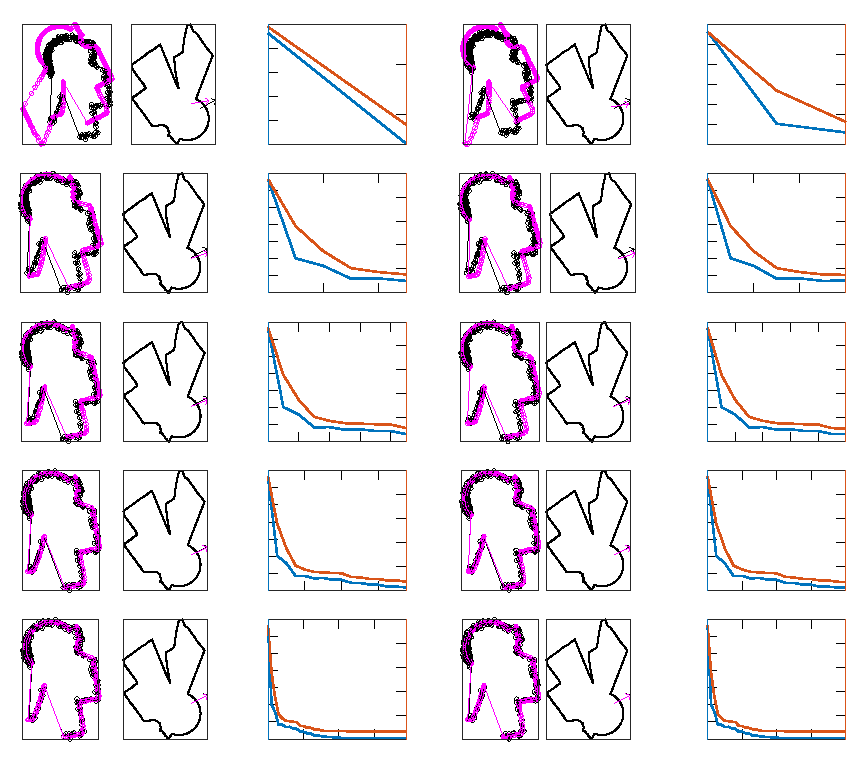
\includegraphics{./figures/parts/02/chapters/04/sections/04/sr5_sm0_1}}%
    \gplfronttext
  \end{picture}%
\endgroup

  \end{subfigure}\\%
  \end{framed}
  \begin{subfigure}{\linewidth}\hspace{-0.25cm}
    % GNUPLOT: LaTeX picture with Postscript
\begingroup
  \makeatletter
  \providecommand\color[2][]{%
    \GenericError{(gnuplot) \space\space\space\@spaces}{%
      Package color not loaded in conjunction with
      terminal option `colourtext'%
    }{See the gnuplot documentation for explanation.%
    }{Either use 'blacktext' in gnuplot or load the package
      color.sty in LaTeX.}%
    \renewcommand\color[2][]{}%
  }%
  \providecommand\includegraphics[2][]{%
    \GenericError{(gnuplot) \space\space\space\@spaces}{%
      Package graphicx or graphics not loaded%
    }{See the gnuplot documentation for explanation.%
    }{The gnuplot epslatex terminal needs graphicx.sty or graphics.sty.}%
    \renewcommand\includegraphics[2][]{}%
  }%
  \providecommand\rotatebox[2]{#2}%
  \@ifundefined{ifGPcolor}{%
    \newif\ifGPcolor
    \GPcolorfalse
  }{}%
  \@ifundefined{ifGPblacktext}{%
    \newif\ifGPblacktext
    \GPblacktexttrue
  }{}%
  % define a \g@addto@macro without @ in the name:
  \let\gplgaddtomacro\g@addto@macro
  % define empty templates for all commands taking text:
  \gdef\gplfronttext{}%
  \gdef\gplfronttext{}%
  \makeatother
  \ifGPblacktext
    % no textcolor at all
    \def\colorrgb#1{}%
    \def\colorgray#1{}%
  \else
    % gray or color?
    \ifGPcolor
      \def\colorrgb#1{\color[rgb]{#1}}%
      \def\colorgray#1{\color[gray]{#1}}%
      \expandafter\def\csname LTw\endcsname{\color{white}}%
      \expandafter\def\csname LTb\endcsname{\color{black}}%
      \expandafter\def\csname LTa\endcsname{\color{black}}%
      \expandafter\def\csname LT0\endcsname{\color[rgb]{1,0,0}}%
      \expandafter\def\csname LT1\endcsname{\color[rgb]{0,1,0}}%
      \expandafter\def\csname LT2\endcsname{\color[rgb]{0,0,1}}%
      \expandafter\def\csname LT3\endcsname{\color[rgb]{1,0,1}}%
      \expandafter\def\csname LT4\endcsname{\color[rgb]{0,1,1}}%
      \expandafter\def\csname LT5\endcsname{\color[rgb]{1,1,0}}%
      \expandafter\def\csname LT6\endcsname{\color[rgb]{0,0,0}}%
      \expandafter\def\csname LT7\endcsname{\color[rgb]{1,0.3,0}}%
      \expandafter\def\csname LT8\endcsname{\color[rgb]{0.5,0.5,0.5}}%
    \else
      % gray
      \def\colorrgb#1{\color{black}}%
      \def\colorgray#1{\color[gray]{#1}}%
      \expandafter\def\csname LTw\endcsname{\color{white}}%
      \expandafter\def\csname LTb\endcsname{\color{black}}%
      \expandafter\def\csname LTa\endcsname{\color{black}}%
      \expandafter\def\csname LT0\endcsname{\color{black}}%
      \expandafter\def\csname LT1\endcsname{\color{black}}%
      \expandafter\def\csname LT2\endcsname{\color{black}}%
      \expandafter\def\csname LT3\endcsname{\color{black}}%
      \expandafter\def\csname LT4\endcsname{\color{black}}%
      \expandafter\def\csname LT5\endcsname{\color{black}}%
      \expandafter\def\csname LT6\endcsname{\color{black}}%
      \expandafter\def\csname LT7\endcsname{\color{black}}%
      \expandafter\def\csname LT8\endcsname{\color{black}}%
    \fi
  \fi
    \setlength{\unitlength}{0.0500bp}%
    \ifx\gptboxheight\undefined%
      \newlength{\gptboxheight}%
      \newlength{\gptboxwidth}%
      \newsavebox{\gptboxtext}%
    \fi%
    \setlength{\fboxrule}{0.5pt}%
    \setlength{\fboxsep}{1pt}%
\begin{picture}(8000.00,2600.00)%
    \gplgaddtomacro\gplfronttext{%
      \colorrgb{0.15,0.15,0.15}%
      \put(1425,260){\makebox(0,0)[r]{\strut{}$1.0$}}%
      \colorrgb{0.15,0.15,0.15}%
      \put(1425,854){\makebox(0,0)[r]{\strut{}$2.0$}}%
      \colorrgb{0.15,0.15,0.15}%
      \put(1425,1448){\makebox(0,0)[r]{\strut{}$3.0$}}%
      \colorrgb{0.15,0.15,0.15}%
      \put(1425,2042){\makebox(0,0)[r]{\strut{}$4.0$}}%
      \colorrgb{0.15,0.15,0.15}%
      \put(1854,40){\makebox(0,0){\strut{}$-1.0$}}%
      \colorrgb{0.15,0.15,0.15}%
      \put(2448,40){\makebox(0,0){\strut{}$0$}}%
      \colorrgb{0.15,0.15,0.15}%
      \put(3042,40){\makebox(0,0){\strut{}$1.0$}}%
    }%
    \gplgaddtomacro\gplfronttext{%
    }%
    \gplgaddtomacro\gplfronttext{%
      \colorrgb{0.15,0.15,0.15}%
      \put(4676,557){\makebox(0,0)[r]{\strut{}$-2.0$}}%
      \colorrgb{0.15,0.15,0.15}%
      \put(4676,1151){\makebox(0,0)[r]{\strut{}$-1.0$}}%
      \colorrgb{0.15,0.15,0.15}%
      \put(4676,1745){\makebox(0,0)[r]{\strut{}$0$}}%
      \colorrgb{0.15,0.15,0.15}%
      \put(4676,2339){\makebox(0,0)[r]{\strut{}$1.0$}}%
      \colorrgb{0.15,0.15,0.15}%
      \put(4808,40){\makebox(0,0){\strut{}$-1.0$}}%
      \colorrgb{0.15,0.15,0.15}%
      \put(5402,40){\makebox(0,0){\strut{}$0$}}%
      \colorrgb{0.15,0.15,0.15}%
      \put(5996,40){\makebox(0,0){\strut{}$1.0$}}%
      \colorrgb{0.15,0.15,0.15}%
      \put(6590,40){\makebox(0,0){\strut{}$2.0$}}%
    }%
    \gplgaddtomacro\gplfronttext{%
      \put(2299,2559){\makebox(0,0){\strut{}Τελική εκτίμηση}}%
      \put(5699,2559){\makebox(0,0){\strut{}Τελική ευθυγράμμιση}}%
    }%
    \put(0,0){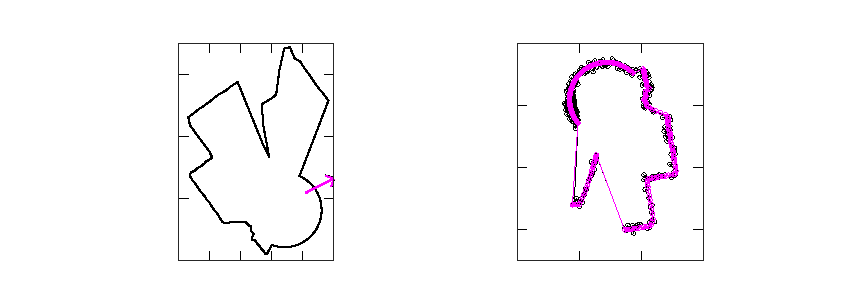
\includegraphics{./figures/parts/02/chapters/04/sections/04/sr5_sm0_2}}%
    \gplfronttext
  \end{picture}%
\endgroup

  \end{subfigure}%
  \caption{}
  \label{}
\end{figure}
